\documentclass[a4paper, 10pt]{report}

\usepackage{fullpage}
\usepackage{minted}
\usepackage[utf8]{inputenc}
\usepackage[english]{babel}
\usepackage{latexsym}
\usepackage{amssymb}
\usepackage{amsmath}
\usepackage{amsthm}
\usepackage{mathpartir}
\usepackage{epsfig}
\usepackage[T1]{fontenc}
\usepackage{stmaryrd}
\usepackage{color}
\usepackage{epstopdf}
\usepackage{microtype}
\usepackage{hyperref}
\usepackage[en-GB]{datetime2}
\DTMlangsetup[en-GB]{showdayofmonth=false}
\usepackage{lipsum}
\usepackage{caption}
\usepackage{subcaption}
\usepackage{iris}
\usepackage{heaplang}
\usepackage{tikz}
\usetikzlibrary{calc,shapes.multipart,chains,arrows}
\usepackage{xspace}
\usepackage{lineno}
\usepackage{booktabs}
\usepackage{tabularx}
\usepackage{multirow}
\usepackage{adjustbox}
\usepackage{csquotes}

\renewcommand*\sfdefault{lmss}
\renewcommand*\ttdefault{txtt}
\definecolor{codebg}{HTML}{f0f0f0}

% Theorems, Corollaries, and Lemmas
\theoremstyle{definition}
\newtheorem{theorem}{Theorem}
\newtheorem{corollary}{Corollary}[theorem]
\newtheorem{lemma}[theorem]{Lemma}

\newtheorem{definition}{Definition}[section]


\newcommand{\isLock}{\operatorname{isLock}}
\newcommand{\locked}{\operatorname{locked}}
\newcommand{\issued}{\operatorname{issued}}
\newcommand{\newLock}{\operatorname{newLock}}
\newcommand{\acquire}{\operatorname{acquire}}
\newcommand{\wait}{\operatorname{wait}}
\newcommand{\release}{\operatorname{release}}
\newcommand{\lockInv}{\operatorname{lockInv}}
\newcommand{\initialise}{\operatorname{initialize}}
\newcommand{\enqueue}{\operatorname{enqueue}}
\newcommand{\dequeue}{\operatorname{dequeue}}

\newcommand{\msq}{M\&S-Queue\xspace}
\newcommand{\tlmsq}{Two-Lock \msq}
\newcommand{\lfmsq}{Lock-Free \msq}

\newcommand{\isqueue}{\operatorname{is\_queue}}
\newcommand{\isqueueseq}{\operatorname{is\_queue\_seq}}
\newcommand{\isqueueconc}{\operatorname{is\_queue\_conc}}
\newcommand{\TLQueueInvariantConc}{\operatorname{I_{TLC}}}
\newcommand{\TLQueueInvariantHocap}{\operatorname{I_{TLH}}}
\newcommand{\LFQueueInvariantHocap}{\operatorname{I_{LFH}}}
\newcommand{\SeqQgnames}{SeqQgnames}
\newcommand{\ConcQgnames}{ConcQgnames}
\newcommand{\Qgnames}{Qgnames}

\newcommand{\vq}{v_q}
\newcommand{\xsc}{xs}
\newcommand{\xsqueue}{xs_{\mathrm{queue}}}
\newcommand{\xsold}{xs_{\mathrm{old}}}

\newcommand{\isLLchain}{\operatorname{isLL\_chain}}
\newcommand{\isLL}{\operatorname{isLL}}
\newcommand{\AllP}{\operatorname{All}}
\newcommand{\projval}{\operatorname{proj\_val}}
\newcommand{\wrapsome}{\operatorname{wrap\_some}}
\newcommand{\isLast}{\operatorname{isLast}}
\newcommand{\isSndLast}{\operatorname{isSndLast}}
\newcommand{\projqgnamesseq}{\operatorname{proj\_Qgnames\_seq}}
\newcommand{\projqgnamesconc}{\operatorname{proj\_Qgnames\_conc}}

\newcommand{\locin}{\loc_{\mathrm{in}}}
\newcommand{\locinM}[1]{\loc_{#1\_\mathrm{in}}}
\newcommand{\locout}{\loc_{\mathrm{out}}}
\newcommand{\locoutM}[1]{\loc_{#1\_\mathrm{out}}}

\newcommand{\locN}[1]{\loc_{\mathrm{#1}}}
\newcommand{\lochead}{\locN{head}}
\newcommand{\loctail}{\locN{tail}}
\newcommand{\locqueue}{\locN{queue}}

\newcommand{\nodeval}{\valB}
\newcommand{\nodevalM}[1]{\nodeval_{#1}}

\newcommand{\nIn}[1]{\operatorname{in}(#1)}
\newcommand{\nVal}[1]{\operatorname{val}(#1)}
\newcommand{\nOut}[1]{\operatorname{out}(#1)}

\newcommand{\node}{x}
\newcommand{\nodeM}[1]{\node_{#1}}
\newcommand{\nodeN}[1]{\node_{\mathrm{#1}}}
\newcommand{\nodehead}{\nodeN{head}}
\newcommand{\nodetail}{\nodeN{tail}}
\newcommand{\nodelast}{\nodeN{last}}
\newcommand{\nodenew}{\nodeN{new}}
\newcommand{\nodeheadnext}{\nodeN{head\_next}}
\newcommand{\nodetailnext}{\nodeN{tail\_next}}
\newcommand{\nodenewtail}{\nodeN{newtail}}

\newcommand{\absvalue}{\val}
\newcommand{\absvalueList}{xs_v}

\newcommand{\Hlock}{h_{\mathrm{lock}}}
\newcommand{\Tlock}{t_{\mathrm{lock}}}
\newcommand{\Hlockvar}{H\_lock}
\newcommand{\Tlockvar}{T\_lock}

\newcommand{\prophval}{\val_p}

\newcommand{\StaticState}{\textbf{Static}\xspace}
\newcommand{\EnqueueState}{\textbf{Enqueue}\xspace}
\newcommand{\DequeueState}{\textbf{Dequeue}\xspace}
\newcommand{\BothState}{\textbf{Both}\xspace}

\newcommand{\Qg}{Q_\gname}
\newcommand{\Qgseq}{Q_{\gname S}}
\newcommand{\Qgconc}{Q_{\gname C}}
\newcommand{\Qghocap}{Q_{\gname H}}

\newcommand{\ghlock}{\gname_{\mathrm{Hlock}}}
\newcommand{\gtlock}{\gname_{\mathrm{Tlock}}}
\newcommand{\gabst}{\gname_{\mathrm{Abst}}}
\newcommand{\ghead}{\gname_{\mathrm{Head}}}
\newcommand{\gtail}{\gname_{\mathrm{Tail}}}
\newcommand{\glast}{\gname_{\mathrm{Last}}}

\newcommand{\TokE}[1]{\operatorname{TokE} ~ #1}
\newcommand{\TokEQg}{\TokE{\Qg}}
\newcommand{\ToknE}[1]{\operatorname{ToknE} ~ #1}
\newcommand{\ToknEQg}{\ToknE{\Qg}}
\newcommand{\TokD}[1]{\operatorname{TokD} ~ #1}
\newcommand{\TokDQg}{\TokD{\Qg}}
\newcommand{\ToknD}[1]{\operatorname{ToknD} ~ #1}
\newcommand{\ToknDQg}{\ToknD{\Qg}}
\newcommand{\TokBefore}[1]{\operatorname{TokBefore} ~ #1}
\newcommand{\TokBeforeQg}{\TokBefore{\Qg}}
\newcommand{\TokAfter}[1]{\operatorname{TokAfter} ~ #1}
\newcommand{\TokAfterQg}{\TokAfter{\Qg}}
\newcommand{\TokUpdated}[1]{\operatorname{TokUpdated} ~ #1}
\newcommand{\TokUpdatedQg}{\TokUpdated{\Qg}}

\newcommand\catenate{\mathbin{\text{\ttfamily\upshape ++}}}

\newcommand{\BB}{\ensuremath{\mathbb{B}}}
\newcommand{\Cc}{\ensuremath{\mathbf{C}}}
\newcommand{\El}{\ensuremath{\mathcal{E}}}
\newcommand{\Sl}{\ensuremath{\mathcal{S}}}
\newcommand{\Ul}{\ensuremath{\mathcal{U}}}
\newcommand{\Dl}{\ensuremath{\mathcal{D}}}
\newcommand{\Fl}{\ensuremath{\mathcal{F}}}
\newcommand{\Pl}{\ensuremath{\mathcal{P}}}
\newcommand{\Tl}{\ensuremath{\mathcal{T}}}
\newcommand{\CC}{\ensuremath{\mathbb{C}}}
\newcommand{\KK}{\ensuremath{\mathbb{K}}}
\newcommand{\PP}{\ensuremath{\mathbb{P}}}
\newcommand{\VV}{\ensuremath{\mathbb{V}}}
\newcommand{\UU}{\ensuremath{\mathbb{U}}}
\newcommand{\DD}{\ensuremath{\mathbb{D}}}
\newcommand{\Ml}{\ensuremath{\mathcal{M}}}
\newcommand{\Vl}{\ensuremath{\mathcal{V}}}
\newcommand{\Il}{\ensuremath{\mathcal{I}}}
\newcommand{\Cl}{\ensuremath{\mathcal{C}}}
\newcommand{\Bl}{\ensuremath{\mathcal{B}}}
\newcommand{\Al}{\ensuremath{\mathcal{A}}}
\newcommand{\Gl}{\ensuremath{\mathcal{G}}}
\newcommand{\Nl}{\ensuremath{\mathcal{N}}}
\newcommand{\AAA}{\ensuremath{\mathbb{A}}}
\newcommand{\EE}{\ensuremath{\mathbb{E}}}

\newcommand{\isNode}[1]{\nIn{#1} \mapsto^{\persistently} (\nVal{#1}, \nOut{#1})}

\newcommand{\abstractstatefrac}[3]{#1 \Mapsto\kern-0.5ex\tfrac{1}{#2} #3}
\newcommand{\abstractstate}[3]{#1 \Mapsto^{#2}_{\circ} #3}
\newcommand{\abstractstatefullfrag}[2]{#1 \Mapsto_{\circ} #2}
\newcommand{\abstractstateauth}[2]{#1 \Mapsto_{\bullet} #2}

\newcommand{\reach}[2]{#1 \leadsto #2}
\newcommand{\ar}[2]{#1 \dashrightarrow #2}
\newcommand{\ap}[2]{#1 \rightarrowtail #2}

%%%%%%%%%%%%%%%%%%%%%%%%%%%%%%%%%%%%%%%%%%%%%%%%%%%%%%%%%%%%%%%%%%%%%%%
% Specifications

\newcommand{\tlseqspecinit}{\hoare{\TRUE}{\initialise \ \TT}{\vq . \Exists \Qg. \isqueueseq(\vq, [], \Qg)}}

\newcommand{\tlseqspecenq}{\All \vq, \absvalue, \absvalueList, \Qg. \hoare{\isqueueseq(\vq, \absvalueList, \Qg)}{\enqueue \ \vq \ \absvalue}{\valB . \isqueueseq(\vq, (\absvalue :: \absvalueList), \Qg)}}

\newcommand{\tlseqspecdeq}{\All \vq, \absvalueList, \Qg. \hoareV[t]{\isqueueseq(\vq, \absvalueList, \Qg)}{\dequeue \ \vq}{\nodeval . \begin{array}{l}(\absvalueList = [] \star \nodeval = \None \star \isqueueseq(\vq, \absvalueList, \Qg)) ~ \lor\\ (\Exists \absvalue, \absvalueList' . \absvalueList = \absvalueList' \catenate [\absvalue] \star \nodeval = \Some \absvalue \star \isqueueseq(\vq, \absvalueList', \Qg)) \end{array}}}


\newcommand{\tlconcspecinit}{\hoare{\TRUE}{\initialise \ \TT}{\vq . \Exists \Qg. \isqueueconc(\Phi, \vq, \Qg)}}

\newcommand{\tlconcspecenq}{\All \vq, \absvalue, \Qg. \hoare{\isqueueconc(\Phi,\vq,\Qg) \star \Phi(\absvalue)}{\enqueue \ \vq \ \absvalue}{\valB . \TRUE}}

\newcommand{\tlconcspecdeq}{\All \vq, \Qg. \hoare{\isqueueconc(\Phi, \vq, \Qg)}{\dequeue \ \vq}{\nodeval . \nodeval = \None \lor (\Exists \absvalue. \nodeval = \Some \absvalue \star \Phi(\absvalue))}}


\newcommand{\tlhocapspecinit}{\hoare{\TRUE}{\initialise \ \TT}{\vq . \Exists \Qg . \isqueue(\vq, \Qg) \star \abstractstatefullfrag{\Qg.\gabst}{[]}}}

\newcommand{\tlhocapspecenq}{\All \vq, \absvalue, \Qg, P, Q.
\begin{array}[t]{l}
\left(\All \absvalueList . \abstractstateauth{\Qg.\gabst}{\absvalueList} \star P \vs[\mask\setminus\Nl.i^\uparrow] \later \abstractstateauth{\Qg.\gabst}{\absvalue :: \absvalueList} \star Q \right)
\wand\\
\hoare{\isqueue(\vq, \Qg) \star P}{\enqueue \ \vq \ \absvalue}{\valB . Q}
\end{array}}

\newcommand{\tlhocapspecdeq}{\All \vq, \Qg, P, Q.
\begin{array}[t]{l}
\left(\All \absvalueList . \abstractstateauth{\Qg.\gabst}{\absvalueList} \star P \vs[\mask\setminus\Nl.i^\uparrow] \later
  \left(
    \begin{array}{l}
      (\absvalueList = [] \star \abstractstateauth{\Qg.\gabst}{\absvalueList} \star Q(\None))\\
      \lor
      \left(
        \begin{array}{l}
          \Exists \absvalue, \absvalueList' . \absvalueList = \absvalueList' \catenate [\absvalue] \star\\
          \abstractstateauth{\Qg.\gabst}{\absvalueList'} \star Q(\Some{\absvalue})
        \end{array}
        \right)
    \end{array}
  \right) \right)
\wand\\
\hoare{\isqueue(\vq, \Qg) \star P}{\dequeue \ \vq}{\nodeval . Q(\nodeval)}
\end{array}}


\newcommand{\lfhocapspecinit}{\tlhocapspecinit}

\newcommand{\lfhocapspecenq}{\tlhocapspecenq}

\newcommand{\lfhocapspecdeq}{\tlhocapspecdeq}


%%%%%%%%%%%%%%%%%%%%%%%%%%%%%%%%%%%%%%%%%%%%%%%%%%%%%%%%%%%%%%%%%%%%%%%

\newcommand{\todo}[1]{{\color[rgb]{.5,0,0}\textbf{$\blacktriangleright$#1$\blacktriangleleft$}}}

\begin{document}

%%%%%%%%%%%%%%%%%%%%%%%%%%%%%%%%%%%%%%%%%%%%%%%%%%%%%%%%%%%%%%%%%%%%%%%

\pagestyle{empty}
\pagenumbering{roman}
\vspace*{\fill}\noindent{\rule{\linewidth}{1mm}\\[4ex]
{\Huge\sf Verification of the Blocking and Non-Blocking Michael-Scott Queue Algorithms}\\[2ex]
{\huge\sf Mathias Pedersen, 201808137}\\[2ex]
\noindent\rule{\linewidth}{1mm}\\[4ex]
\noindent{\Large\sf Master's Thesis, Computer Science\\[1ex]
\today \\[1ex] Advisor: Amin Timany\\[15ex]}\\[\fill]}
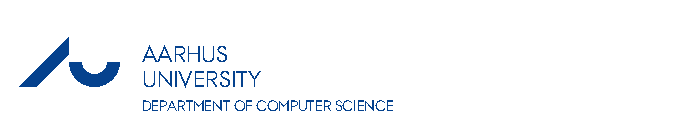
\epsfig{file=logo.eps}\clearpage

%%%%%%%%%%%%%%%%%%%%%%%%%%%%%%%%%%%%%%%%%%%%%%%%%%%%%%%%%%%%%%%%%%%%%%%

\pagestyle{plain}
\chapter*{Abstract}
\addcontentsline{toc}{chapter}{Abstract}

\todo{in English\dots}

\chapter*{Resum\'e}
\addcontentsline{toc}{chapter}{Resum\'e}

\todo{in Danish\dots}

\chapter*{Acknowledgments}
\addcontentsline{toc}{chapter}{Acknowledgments}

\todo{\dots}

\vspace{2ex}
\begin{flushright}
  \emph{Mathias Pedersen}\\
  \emph{Aarhus, \today.}
\end{flushright}

\tableofcontents
\cleardoublepage
\pagenumbering{arabic}
\setcounter{secnumdepth}{2}

%%%%%%%%%%%%%%%%%%%%%%%%%%%%%%%%%%%%%%%%%%%%%%%%%%%%%%%%%%%%%%%%%%%%%%%

\chapter{Introduction}
\label{ch:intro}

\todo{motivate and explain the problem to be addressed}

\todo{example of a citation: \cite{DBLP:conf/podc/MichaelS96}}
\todo{get your bibtex entries from \url{https://dblp.org/}}
\todo{Emphasise that specs for two-lock and lock-free are equivalent, with only the queue functions being different. This is even shown in the coq proofs}
\todo{Have a bullet point list of contributions}


\todo{direct specifications for TL and LF Queues (instead of refinement)}
\todo{Add more contributions}



%%%%%%%%%%%%%%%%%%%%%%%%%%%%%%%%%%%%%%%%%%%%%%%%%%%%%%%%%%%%%%%%%%%%%%%

\chapter{Preliminaries}
\label{ch:preliminaries}

\todo{Mention that the project uses heaplang and the program logic iris, and hence we need to know about them}


\section{\heaplang}
\label{Pre:section:heaplang}

\todo{Write about heaplang language: ml like, with a heap, Cas}
\todo{Refer to ILN for specification}
\todo{Talk about Syntactic sugar: i.e. e1 ;; e2 = (lam v, e2) e1 where v is fresh, and CAS ... as Snd (CMPXHG ...), and derived rules for them}
\todo{also mention prophecies and refer to the section talking about them}


\section{The Iris Program Logic Framework}
\label{Pre:section:iris}
In this section, we give a brief introduction to Iris -- the logic we use to reason about the \msq's. Iris is quite expressive and supports a myriad of features and derived rules, many of which have been utilised in this project. As such, it will be impossible to cover all facets of Iris in detail, so we limit ourselves to give an overview of the main aspects of Iris. If the reader wishes a more thorough introduction, or wants to see further details of the topics covered, please consult the Iris Lecture Notes \cite{gentleiris}.

\todo{FOCUS IN THIS SECTION is on explaining the basic ideas of the concepts and showing the notation used. Assume the reader is somewhat familiar with program verification. }

\subsection{Fundamentals of Iris}
\todo{program logic framework}
\todo{instantiate with a language, here heaplang}
\todo{higher order logic}
\todo{seperation logic}
\todo{- exclusive ownership and duplicability}
\todo{introduce persistent modality, duplicability}
\todo{points-to predicates}
\todo{resource oriented}
\todo{derivation rules examples...}

\subsection{Hoare Triples and Weakest Pre-Condition}
\todo{explain hoare triples}
\todo{talk about Partial correctness and Adequacy}
\todo{explain weakest pre-conditions}
\todo{show how they are related}

\subsection{Later Modality}
\todo{explain concept}
\todo{ties propositions to program steps}
\todo{Explain the löb induction rule, mention the intuition when P is hoare triple}

The later modality adds a notion of step indexing to Iris propositions. This step indexing is technically parallel to the notion of taking steps in the programs, but the way we define hoare-triples and weakest-preconditions tie program steps together with steps in the logic. In other words, a single Later corresponds to a single step in the program.

\subsection{Invariants}
\todo{explain the idea}
\todo{open around atomic expression}
\todo{only one opening at a time}
\todo{namespaces}
\todo{Show the basic rules. Inv-alloc (FUP), ...}

\subsection{Resource Algebra}
\todo{Introduce the idea}
\todo{Validity}
\todo{introduce $\mtimes$ and $\mincl$}
\todo{tying them into the logic}
  \todo{also ghost names}
  \todo{own-allocate own-op, own-valid...}
\todo{mention that points-to predicate is also a resource algebra}
\todo{composing resource algebras}
\todo{we introduce the resource algebras we use at the point of use}

\subsection{Update modality and Viewshift}
\todo{explain the ideas}


\section{Formalisation in Coq}
\label{Pre:section:coq}

Iris has been mechanised in the Coq proof assistant\footnote{The mechanisation can be found at \url{https://gitlab.mpi-sws.org/iris/iris/}} -- a tool to machine-check proofs of mathematical assertions. All results in this project have been completely machine-verified in the Iris mechanisation in Coq. Specifications in the Coq formalisation of Iris are usually written in terms of hoare-triples but proved by first converting the hoare-triples to equivalent weakest-preconditions, as this is usually easier to work with. The proofs presented in this report will follow suit and give specifications using hoare-triples, but prove them assuming they are weakest-preconditions. The proofs presented in the report thus follow the mechanised proofs very closely, making it possible to ``step-through'' the mechanised proofs in tandem with reading the paper-proofs presented in this report.

One caveat is that, although the theory discussed in the previous section remain valid, the underlying model of Iris is somewhat more complex than the section presented it to be. Working with the Coq formalisation of Iris thus requires a bit deeper understanding of the model of Iris. \cite{DBLP:journals/jfp/JungKJBBD18} explains the underlying model of an older version of Iris, but many of the concepts discussed are still relevant\footnote{For an up-to-date presentation, please consult the Technical Reference at \url{https://iris-project.org/}}.

Table \ref{Pre:files-table} gives an overview over the files developed in the project and how they relate to this report. All files related to the project are available at \url{https://github.com/MatteP1/thesis}.

\begin{table}[h]
\begin{adjustbox}{center}
\begin{tabularx}{\textwidth}{llX}
  \toprule
  \textbf{File Name} & \textbf{Relevant Sections} & \textbf{Description} \\
  \midrule
  \path{MSQ_common.v} & Chapters \ref{ch:TLMSQ} - \ref{ch:LFMSQ} & Common definitions and lemmas. \\
  \midrule
  \path{twoLockMSQ_impl.v} & Chapter \ref{ch:TLMSQ} & \multirow{5}{\linewidth}{\tlmsq implementation and proofs of three specifications. Two of them shown to be derivable from the third.} \\
  \path{twoLockMSQ_sequential_spec.v} & Chapter \ref{ch:TLMSQSEQ} & \\
  \path{twoLockMSQ_concurrent_spec.v} & Chapter \ref{ch:TLMSQCONC} & \\
  \path{twoLockMSQ_hocap_spec.v} & Chapter \ref{ch:TLMSQHOCAP}& \\
  \path{twoLockMSQ_derived.v} & Section \ref{TLMSQHOCAP:section:deriving-seq-and-conc} & \\
  \midrule
  \path{lockFreeMSQ_impl.v} & Section \ref{LFMSQ:section:implementation} & \multirow{3}{\linewidth}{\lfmsq implementation and Hocap-style + derived specifications.} \\
  \path{lockFreeMSQ_hocap_spec.v} & Sections \ref{LFMSQ:section:reachability} - \ref{LFMSQ:section:proof-outline} & \\
  \path{lockFreeMSQ_derived.v} & Sections \ref{LFMSQ:section:spec} and \ref{TLMSQHOCAP:section:deriving-seq-and-conc} & \\
  \midrule
  \path{lockAndCCFreeMSQ_impl.v} & Section \ref{LFMSQ:section:discussion} & \multirow{2}{\linewidth}{Consistency-Check-Free version of \lfmsq.}\\
  \path{lockAndCCFreeMSQ_hocap_spec.v} & Section \ref{LFMSQ:section:discussion}& \\
  \midrule
  \path{queue_specs.v} & N/A & Implementation-independent specs. \\
  \bottomrule
\end{tabularx}
\end{adjustbox}
\caption{Overview of Coq Files}
\label{Pre:files-table}
\end{table}

\subsection{Compiling the Project}
Compiling the project (on \linuxname) requires both Coq and Iris to be installed. Once installed, open a terminal and navigate to the project folder, containing \path{_CoqProject}. Then run the following two commands, which (1) generates a makefile and (2) runs the makefile.
\begin{minted}[style=friendly, bgcolor=codebg, linenos]{shell-session}
  $ coq_makefile -f _CoqProject -o CoqMakefile
  $ make -f CoqMakefile
\end{minted}
The project is known to compile with Coq version 8.19.0 and Iris version 4.2.0.


\chapter{The Two-Lock Michael Scott Queue}
\label{ch:TLMSQ}

In this chapter, we give an implementation of the blocking version of the \msq, the \tlmsq, in \heaplang. This implementation differs slightly from the original, presented in \cite{DBLP:conf/podc/MichaelS96}, but most changes simply reflect the differences in the two languages.


\section{Introduction}
\label{TLMSQ:section:introduction}

The underlying data structure making up the queue is a singly-linked list. The linked-list will always contain at least one element, called the \emph{head} node, marking the beginning of the queue. Note that the head node is itself not part of the queue, but all nodes following it are. The queue keeps a head pointer ($\lochead$) which always points to the head node, and a tail pointer ($\loctail$) which points to some node in the linked list, denoted the tail node.

In my implementation, a node is a triple $(\locinM{i}, \nodevalM{i}, \locoutM{i})$ satisfying that location $\locinM{i}$ points to the pair $(\nodevalM{i}, \locoutM{i})$. Here, $\nodevalM{i}$ either contains the value of the node $\absvalue_i$ wrapped in a $\Some$ (i.e. $\nodevalM{i} = \Some \absvalue_i$) or it is $\None$. $\locoutM{i}$ either points to $\None$ which represents the null pointer, or to the next node in the linked list. When we say that a location $\loc$ points to a node $(\locinM{i}, \nodevalM{i}, \locoutM{i})$, we mean that $\loc \mapsto \locinM{i}$. Hence, if we have two adjacent nodes $(\locinM{i}, \nodevalM{i}, \locoutM{i})$, $(\locinM{i+1}, \nodevalM{i+1}, \locoutM{i+1})$ in the linked list, then we have the following structure: $\locinM{i} \mapsto (\nodevalM{i}, \locoutM{i})$, $\locoutM{i} \mapsto \locinM{i+1}$, and $\locinM{i+1} \mapsto \nodevalM{i+1}, \locoutM{i+1}$.
For a given triple $\node = (\locin, \nodeval, \locout)$, we introduce the following notation:
\begin{align*}
  &\nIn{\node} = \locin& &\nVal{\node} = \nodeval& &\nOut{\node} = \locout
\end{align*}

The reader may wonder why there is an extra, intermediary ``in'' pointer, between the pairs of the linked list, and why the ``out'' pointer couldn't point directly to the next pair. In the original implementation \cite{DBLP:conf/podc/MichaelS96}, nodes are allocated on the heap. To simulate this in \heaplang, when creating a new node, we create a pointer to a pair making up the node. Now, in the C-like language used in the original specification, an assignment operator is available which is not present in \heaplang. So in order to mimic this behaviour, we model variables as pointers. In this way, we can model a variable $\lvarA$ as a location $\loc_{\lvarA}$, and the value stored at $\loc_{\lvarA}$ is the current value of $\lvarA$. This means that the variable ``next'' in the original implementation becomes a location $\locout$, and the value stored at the location is what it is currently assigned to. Since ``next'' is supposed to be a variable containing a pointer, then the value that $\locout$ points to will also be a pointer.


\section{Implementation}
\label{TLMSQ:section:implementation}

The queue consists of 3 functions: $\initialise$, $\enqueue$, and $\dequeue$, and as the name of the data structure suggests, the functions rely on two locks. To this end, we shall assume that we have some lock implementation given. In the accompanying Coq mechanisation, a ``spin-lock'' is used, but the only part we really care about is its specification; this can be found in \cite{gentleiris} (Example 8.38 at the time of writing).

\subsection{Initialise}

$\initialise$ will first create a single node -- the head node -- marking the start of the linked list. It then creates two locks, $\Hlock$ and $\Tlock$, protecting the head and tail pointers, respectively. Finally, it creates the head and tail pointers, both pointing to the head node. The queue is then a pointer to a structure containing the head and tail pointers, and the two locks.

Figure \ref{TLMSQ:impl:figure:init} illustrates the structure of the queue after initialisation. Note that one of the pointers is coloured blue. This represents a \emph{persistent} pointer; a pointer that will never be updated again. All ``in'' pointers $\locinM{i}$, are persistent, meaning that, once created, they will only ever point to $(\nodevalM{i}, \locoutM{i})$. We shall use the notation $\loc \mapsto^{\persistently} \val$ (introduced in \cite{DBLP:conf/cpp/VindumB21}) to mean that $\loc$ points persistently to $\val$.

Note that in the original specification, a queue is a pointer to a 4-tuple $(\lochead, \loctail, \Hlock, \Tlock)$. Since \heaplang doesn't support 4-tuples, we instead represent the queue as a pointer to a pair of pairs: $\left((\lochead, \loctail), (\Hlock, \Tlock)\right)$.

\subsection{Enqueue}

To enqueue a value, we must create a new node, append it to the underlying linked-list, and swing the tail pointer to this new node. These three operations are depicted in figure \ref{TLMSQ:impl:figure:enqueue}.

$\enqueue$ takes as argument the value to be enqueued and creates a new node containing this value (corresponding to figure \ref{TLMSQ:impl:figure:enqueue:a}). This creation doesn't interact with the underlying queue data-structure, hence why we don't acquire $\Tlock$ first. After creating the new node, we must make the last node in the linked list point to it. Since this operation interacts with the queue, we first acquire $\Tlock$. Once we obtain the lock, we make the last node in the linked list point to our new node (figure \ref{TLMSQ:impl:figure:enqueue:b}). Following this, we swing $\loctail$ to the newly inserted node (figure \ref{TLMSQ:impl:figure:enqueue:c}).

Figure \ref{TLMSQ:impl:figure:enqueue} also illustrates when pointers become persistent; once the previous last node is updated to point to the newly inserted node, that pointer will never be updated again, hence becoming persistent.

\subsection{Dequeue}

It is of course only possible to dequeue an element from the queue if the queue contains at least one element. Hence, the first thing $\dequeue$ does is check if the queue is empty. We can detect an empty queue by checking if the head node is the last node in the linked list. Being the last node in the linked list corresponds to having the ``out'' node be $\None$. If this is the case, then the queue is empty and the function returns $\None$. Otherwise, there is a node just after the head node, which is the first node of the queue. To dequeue it, we first read the associated value, and next we swing the head pointer to it, making it the new head node. Finally, we return the value we read.

Since all of these operations interact with the queue, we shall only perform them after having acquired $\Hlock$.

Figure \ref{TLMSQ:impl:figure:dequeue} illustrates running dequeue on a non-empty queue. Note that the only change is that the head pointer is swung to the next node in the linked list; the old head node is not deleted, it just becomes unreachable from the head pointer. In this way, the linked list only ever grows.

\begin{figure}
  \centering
  \begin{adjustbox}{center}
  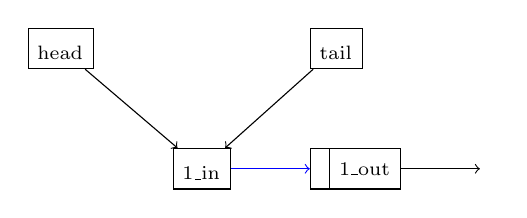
\begin{tikzpicture}[
    pair/.style = {
      on chain,
      rectangle split,
      rectangle split horizontal,
      rectangle split parts=2,
      draw,
      anchor=center,
      text height=1.5ex,
    },
    perspointer/.style = {
      on chain,
      rectangle,
      draw,
      anchor=center,
      text height=1.5ex,
    },
    pointer/.style = {
      rectangle,
      draw,
      anchor=center,
      text height=1.5ex,
    },
    start chain=going right,
  ]

  % Linked List
  \node (l'1) [join={by ->}, perspointer,on chain] {$\locinM{1}$};
  \node (l1pair) [join={by ->, draw=blue}, pair,on chain] {$\None$ \nodepart{two} $\locoutM{1}$};
  \node (null) [join={by ->, draw=black}, rectangle,on chain] {$\None$};

  % Head and tail
  \node (head) [pointer, above left=of l'1] {$\lochead$};
  \node (tail) [pointer, above right=of l'1] {$\loctail$};
  \draw[->] (head) -- (l'1);
  \draw[->] (tail) -- (l'1);

  \end{tikzpicture}
  \end{adjustbox}
  \caption{Queue after initialisation}
  \label{TLMSQ:impl:figure:init}
\end{figure}


\begin{figure}
  \centering
  \begin{subfigure}{\textwidth}
    \begin{adjustbox}{center}
    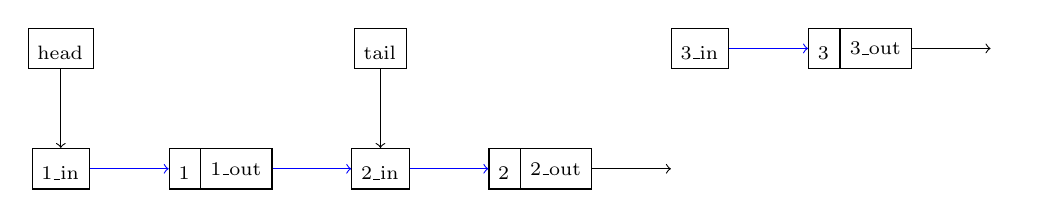
\begin{tikzpicture}[
      pair/.style = {
        on chain,
        rectangle split,
        rectangle split horizontal,
        rectangle split parts=2,
        draw,
        anchor=center,
        text height=1.5ex,
      },
      perspointer/.style = {
        on chain,
        rectangle,
        draw,
        anchor=center,
        text height=1.5ex,
      },
      pointer/.style = {
        rectangle,
        draw,
        anchor=center,
        text height=1.5ex,
      },
      start chain=going right,
    ]

    % Linked List
    \node (l'1) [join={by ->}, perspointer,on chain] {$\locinM{1}$};
    \node (l1pair) [join={by ->, draw=blue}, pair,on chain] {$\nodevalM{1}$ \nodepart{two} $\locoutM{1}$};
    \node (l'2) [join={by ->, draw=blue}, perspointer,on chain] {$\locinM{2}$};
    \node (l2pair) [join={by ->, draw=blue}, pair,on chain] {$\nodevalM{2}$ \nodepart{two} $\locoutM{2}$};
    \node (null) [join={by ->, draw=black}, rectangle,on chain] {$\None$};

    \node (l'3) [perspointer, above right=of l2pair] {$\locinM{3}$};
    \node (l3pair) [join={by ->, draw=blue}, pair,on chain] {$\nodevalM{3}$ \nodepart{two} $\locoutM{3}$};
    \node (null) [join={by ->, draw=black}, rectangle,on chain] {$\None$};

    % Head and tail
    \node (head) [pointer, above=of l'1] {$\lochead$};
    \node (tail) [pointer, above=of l'2] {$\loctail$};
    \draw[->] (head) -- (l'1);
    \draw[->] (tail) -- (l'2);

    \end{tikzpicture}
    \end{adjustbox}
    \caption{Queue after creating the new node $(\locinM{3}, \nodevalM{3}, \locoutM{3})$ to be added to the queue.}
    \label{TLMSQ:impl:figure:enqueue:a}
    \vspace{2em}
  \end{subfigure}
  \begin{subfigure}{\textwidth}
    \begin{adjustbox}{center}
    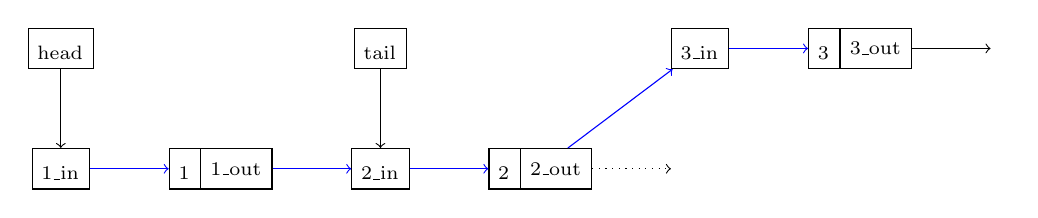
\begin{tikzpicture}[
      pair/.style = {
        on chain,
        rectangle split,
        rectangle split horizontal,
        rectangle split parts=2,
        draw,
        anchor=center,
        text height=1.5ex,
      },
      perspointer/.style = {
        on chain,
        rectangle,
        draw,
        anchor=center,
        text height=1.5ex,
      },
      pointer/.style = {
        rectangle,
        draw,
        anchor=center,
        text height=1.5ex,
      },
      start chain=going right,
    ]

    % Linked List
    \node (l'1) [join={by ->}, perspointer,on chain] {$\locinM{1}$};
    \node (l1pair) [join={by ->, draw=blue}, pair,on chain] {$\nodevalM{1}$ \nodepart{two} $\locoutM{1}$};
    \node (l'2) [join={by ->, draw=blue}, perspointer,on chain] {$\locinM{2}$};
    \node (l2pair) [join={by ->, draw=blue}, pair,on chain] {$\nodevalM{2}$ \nodepart{two} $\locoutM{2}$};
    \node (null) [join={by ->, dotted, draw=black}, rectangle,on chain] {\textcolor{gray}{$\None$}};

    \node (l'3) [perspointer, above right=of l2pair] {$\locinM{3}$};
    \node (l3pair) [join={by ->, draw=blue}, pair,on chain] {$\nodevalM{3}$ \nodepart{two} $\locoutM{3}$};
    \node (null) [join={by ->, draw=black}, rectangle,on chain] {$\None$};
    \draw[->, draw=blue] (l2pair) -- (l'3);

    % Head and tail
    \node (head) [pointer, above=of l'1] {$\lochead$};
    \node (tail) [pointer, above=of l'2] {$\loctail$};
    \draw[->] (head) -- (l'1);
    \draw[->] (tail) -- (l'2);

    \end{tikzpicture}
    \end{adjustbox}
    \caption{Queue after adding the new node to linked list.}
    \label{TLMSQ:impl:figure:enqueue:b}
    \vspace{2em}
  \end{subfigure}
  \begin{subfigure}{\textwidth}
    \begin{adjustbox}{center}
    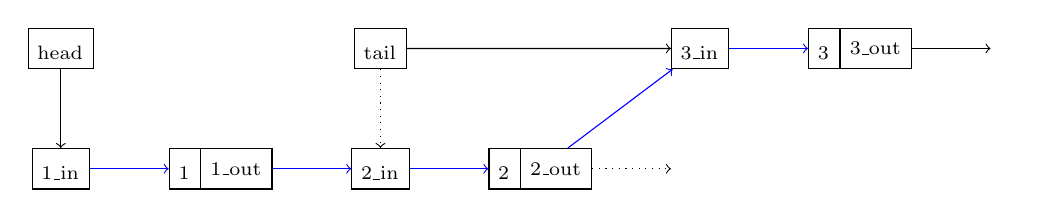
\begin{tikzpicture}[
      pair/.style = {
        on chain,
        rectangle split,
        rectangle split horizontal,
        rectangle split parts=2,
        draw,
        anchor=center,
        text height=1.5ex,
      },
      perspointer/.style = {
        on chain,
        rectangle,
        draw,
        anchor=center,
        text height=1.5ex,
      },
      pointer/.style = {
        rectangle,
        draw,
        anchor=center,
        text height=1.5ex,
      },
      start chain=going right,
    ]

    % Linked List
    \node (l'1) [join={by ->}, perspointer,on chain] {$\locinM{1}$};
    \node (l1pair) [join={by ->, draw=blue}, pair,on chain] {$\nodevalM{1}$ \nodepart{two} $\locoutM{1}$};
    \node (l'2) [join={by ->, draw=blue}, perspointer,on chain] {$\locinM{2}$};
    \node (l2pair) [join={by ->, draw=blue}, pair,on chain] {$\nodevalM{2}$ \nodepart{two} $\locoutM{2}$};
    \node (null) [join={by ->, dotted, draw=black}, rectangle,on chain] {\textcolor{gray}{$\None$}};

    \node (l'3) [perspointer, above right=of l2pair] {$\locinM{3}$};
    \node (l3pair) [join={by ->, draw=blue}, pair,on chain] {$\nodevalM{3}$ \nodepart{two} $\locoutM{3}$};
    \node (null) [join={by ->, draw=black}, rectangle,on chain] {$\None$};
    \draw[->, draw=blue] (l2pair) -- (l'3);

    % Head and tail
    \node (head) [pointer, above=of l'1] {$\lochead$};
    \node (tail) [pointer, above=of l'2] {$\loctail$};
    \draw[->] (head) -- (l'1);
    \draw[->, dotted] (tail) -- (l'2);
    \draw[->] (tail) -- (l'3);

    \end{tikzpicture}
    \end{adjustbox}
    \caption{Queue after swinging tail pointer to the new node.}
    \label{TLMSQ:impl:figure:enqueue:c}
  \end{subfigure}
  \caption{Enqueuing an element to a queue with one element.}
  \label{TLMSQ:impl:figure:enqueue}
\end{figure}


\begin{figure}
  \centering
  \begin{adjustbox}{center}
  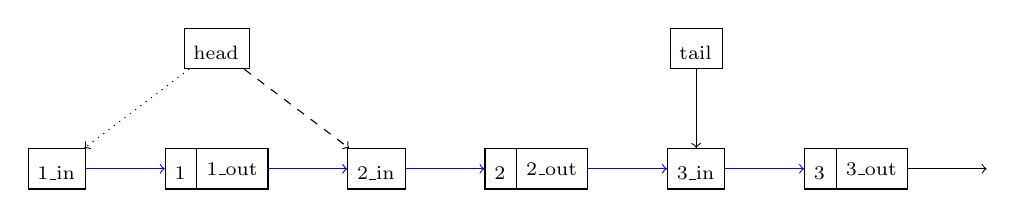
\begin{tikzpicture}[
    pair/.style = {
      on chain,
      rectangle split,
      rectangle split horizontal,
      rectangle split parts=2,
      draw,
      anchor=center,
      text height=1.5ex,
    },
    perspointer/.style = {
      on chain,
      rectangle,
      draw,
      anchor=center,
      text height=1.5ex,
    },
    pointer/.style = {
      rectangle,
      draw,
      anchor=center,
      text height=1.5ex,
    },
    start chain=going right,
  ]

  % Linked List
  \node (l1in) [join={by ->}, perspointer,on chain] {$\locinM{1}$};
  \node (l1pair) [join={by ->, draw=blue}, pair,on chain] {$\nodevalM{1}$ \nodepart{two} $\locoutM{1}$};
  \node (l2in) [join={by ->, draw=blue}, perspointer,on chain] {$\locinM{2}$};
  \node (l2pair) [join={by ->, draw=blue}, pair,on chain] {$\nodevalM{2}$ \nodepart{two} $\locoutM{2}$};
  \node (l3in) [join={by ->, draw=blue}, perspointer,on chain] {$\locinM{3}$};
  \node (l3pair) [join={by ->, draw=blue}, pair,on chain] {$\nodevalM{3}$ \nodepart{two} $\locoutM{3}$};
  \node (null) [join={by ->, draw=black}, rectangle,on chain] {$\None$};

  % Head and tail
  \node (head) [pointer, above=of l1pair] {$\lochead$};
  \node (tail) [pointer, above=of l3in] {$\loctail$};
  \draw[->, dotted] (head) -- (l1in);
  \draw[->, dashed] (head) -- (l2in);
  \draw[->] (tail) -- (l3in);

  \end{tikzpicture}
  \end{adjustbox}
  \caption{Dequeueing an element ($\nodevalM{2}$) from a queue with two elements ($\nodevalM{2}$, $\nodevalM{3}$). The dotted line represents the state before the dequeue, and the dashed line is the state after dequeuing.}
  \label{TLMSQ:impl:figure:dequeue}
\end{figure}

\begin{minted}[linenos=true, escapeinside=||,mathescape=true]{ocaml}
|$\label{TLI:fun}$|  |$ \initialise \eqdef $|
|$\label{TLI:nod}$|    |$ \Let node = \Ref(\None, \Ref(\None)) in $|
|$\label{TLI:hlo}$|    |$ \Let \Hlockvar = \newLock \TT in $|
|$\label{TLI:tlo}$|    |$ \Let \Tlockvar = \newLock \TT in $|
|$\label{TLI:que}$|    |$ \Ref((\Ref(node), \Ref(node)), (\Hlockvar, \Tlockvar)) $|
\end{minted}

\begin{minted}[linenos=true, escapeinside=||,mathescape=true]{ocaml}
|$\label{TLE:fun}$|  |$ \enqueue \ Q \ value \eqdef $|
|$\label{TLE:nod}$|    |$ \Let node = \Ref(\Some value, \Ref(\None)) in $|
|$\label{TLE:acq}$|    |$ \acquire (\Snd (\Snd (\deref Q))); $|
|$\label{TLE:add}$|    |$ \Snd (\deref(\deref(\Snd (\Fst(\deref Q))))) \gets node; $|
|$\label{TLE:sts}$|    |$ \Snd (\Fst (\deref Q)) \gets node; $|
|$\label{TLE:rel}$|    |$ \release (\Snd (\Snd (\deref Q))) $|
\end{minted}

\begin{minted}[linenos=true, escapeinside=||,mathescape=true]{ocaml}
|$\label{TLD:fun}$|  |$ \dequeue \ Q \eqdef $|
|$\label{TLD:acq}$|    |$ \acquire (\Fst (\Snd (\deref Q))); $|
|$\label{TLD:nod}$|    |$ \Let node = \deref (\Fst (\Fst (\deref Q))) in $|
|$\label{TLD:new}$|    |$ \Let new\_head = \deref (\Snd(\deref node)) in $|
|$\label{TLD:ifn}$|    |$ \If new\_head = \None then $|
|$\label{TLD:re1}$|      |$ \release (\Fst (\Snd(\deref Q))); $|
|$\label{TLD:non}$|      |$ \None $|
|$\label{TLD:els}$|    |$ \Else $|
|$\label{TLD:vde}$|      |$ \Let value = \Fst (\deref new\_head) in $|
|$\label{TLD:shs}$|      |$ \Fst (\Fst (\deref Q)) \gets new\_head; $|
|$\label{TLD:re2}$|      |$ \release (\Fst (\Snd (\deref Q))); $|
|$\label{TLD:val}$|      |$ value $|
\end{minted}


\chapter{Sequential Specification}
\label{ch:TLMSQSEQ}

\section{Defining a Sequential Specification}
\label{TLMSQSEQ:section:sequential-spec}

Let us first prove a specification for the \tlmsq in the simple case where we don't allow for concurrency. In this case, we know that only a single thread will interact with the queue at any given point in a sequential manner. The specification we give will track the exact contents of the queue. To this end, we shall define the abstract state of the queue, denoted $\absvalueList$ as a list of \heaplang values. I.e. $\absvalueList : \List ~ \Val$. We adopt the convention that enqueueing an element is done by adding it to the front of the list, and dequeueing removes the last element of the list (if such an element exists). The reason for this choice is purely technical.

Since the queue uses two locks, we will need two ghost names; one for each lock (see specification of lock). For this specification, these are the only two ghost names we will need. However, for the later specifications, we will use more resource algebra, and will need more ghost names. Thus, to ease notation, we shall define the type ``$\SeqQgnames$'' whose purpose is to keep track of the ghost names used for a specific queue. Since we only have two ghost names for this specification, elements of $\SeqQgnames$ will simply be pairs of ghost names. For an element $\Qg \in \SeqQgnames$, the first element of the pair, written $\Qg.\ghlock$, will contain the ghost name for the head lock, and the second element, $\Qg.\gtlock$, the ghost name for the tail lock.

The sequential specification we wish to prove is the following.
\begin{lemma}[\tlmsq Sequential Specification]\label{TLMSQ:spec:seq}
\begin{align*}
  &\Exists \isqueueseq : \Val \to \List ~ \Val \to \SeqQgnames \to \Prop.\\
  &\quad\quad\tlseqspecinit\\
  &\land\quad\tlseqspecenq\\
  &\land\quad\tlseqspecdeq
\end{align*}
\end{lemma}

The proposition $\isqueueseq(\vq, \absvalueList, \Qg)$ captures that the value $\vq$ is a queue, whose content matches that of our abstract representation $\absvalueList$, and the queue uses the ghost names described by $\Qg$. Note that the $\isqueueseq$ predicate is not required to be persistent, hence it cannot be duplicated and given to multiple threads. This is the sense in which this specification is sequential.

\section{Sequential Queue Predicate}
\label{TLMSQSEQ:section:seq-queue-pred}

To prove the specification, we must give a specific $\isqueueseq$ predicate. To help guide us in designing this, we give the following observations about the behaviour of the implementation.
\begin{enumerate}
  \item\label{TLMSQ:insights:head} The head node always points to the first node in the queue (or $\None$ if the queue is empty).
  \item\label{TLMSQ:insights:tail} The tail node is always either the last or second last node in the linked list.
  \item\label{TLMSQ:insights:persistent} All but the last pointer in the linked list (the pointer to $\None$) never change.
\end{enumerate}

Observation \ref{TLMSQ:insights:tail} captures the fact that, while enqueueing, a new node is first added to the linked list, and then later the tail pointer is updated to point to the newly added node. Since only one thread can enqueue a node at a time (due to the lock), then the tail pointer will only ever point to the last or second last node. However, in a sequential setting, the tail will always appear to point to the last node, as no one can inspect the queue while the tail points to the second last.

Insight \ref{TLMSQ:insights:persistent} means that we can mark all pointers in the queue, except the pointer to $\None$, as persistent. This is technically not needed in the sequential case, but we will incorporate it now, as we will need it in the concurrent setting anyway.

With these points in mind, we give our definition of the queue predicate for the sequential specification and explain it afterwards.
\begin{definition}[\tlmsq{} - $\isqueueseq$ Predicate]\label{TLMSQ:spec:seq:isqueueseq}
\begin{align*}
  \isqueueseq(\vq, \absvalueList, \Qg) \eqdef
  &\Exists \locqueue, \lochead, \loctail \in \Loc . \Exists \Hlock, \Tlock \in \Val . \\
  &\vq = \locqueue \star \locqueue \mapsto^{\persistently} ((\lochead, \loctail), (\Hlock, \Tlock)) \star\\
  &\Exists \xsqueue \in \List ~ (\Loc \times \Val \times \Loc) . \Exists \nodehead, \nodetail \in (\Loc \times \Val \times \Loc) .\\
	&\projval(\xsqueue) = \wrapsome(\absvalueList) \star\\
	&\isLL (\xsqueue \catenate [\nodehead]) \star\\
	&\lochead \mapsto \nIn{\nodehead} \star\\
	&\loctail \mapsto \nIn{\nodetail} \star \isLast(\nodetail, (\xsqueue \catenate [\nodehead])) \star\\
	&\isLock(\Qg.\ghlock, \Hlock, \TRUE) \star\\
	&\isLock(\Qg.\gtlock, \Tlock, \TRUE)
\end{align*}
\end{definition}

This $\isqueueseq$ predicate states that the value $\vq$ is a location, which persistently points to the structure containing the head and tail pointers, and the two locks. It also connects the abstract state $\absvalueList$ with the concrete state by stating that if you strip away the locations in $\xsqueue$ (achieved by $\projval$) and wrap the values in the abstract state $\absvalueList$ in $\Some$ (achieved by $\wrapsome$), then the lists become equal.

Next, the predicate specifies the concrete state. There is some head node $\nodehead$, which the head points to. This head node and the nodes in $\xsqueue$ form the underlying linked list (specified using the $\isLL$ predicate below). There is also a tail node, which is the last node in the linked list, and the tail points to this node. The proposition $\isLast(\node, \xsc)$ simply asserts the existence of some $\xsc'$, so that $\xsc = \node :: \xsc'$. 

Next, we have the $\isLock$ predicate for our two locks. Since we are in a sequential setting, the locks are superfluous, hence they simply protect $\TRUE$.

The $\isLL$ predicate essentially creates the structure seen in the examples of section \ref{TLMSQ:section:implementation}. It is defined in two steps. Firstly, we create all the persistent pointers in the linked list using the $\isLLchain$ predicate. Note that this in effect makes $\isLLchain(\xsc)$ persistent for all $\xsc$.
\begin{definition}[Linked List Chain Predicate]
  \begin{align*}
    \isLLchain([]) \equiv& \TRUE\\
    \isLLchain([\node]) \equiv& \isNode{\node}\\
    \isLLchain(\node :: \node' :: \xsc) \equiv& \isNode{\node} \star \nOut{\node'} \mapsto^{\persistently} \nIn{\node} \star \isLLchain(\node' :: \xsc)
  \end{align*}
\end{definition}

Then, to define $\isLL$, we add that the last node in the linked list points to $\None$.
\begin{definition}[Linked List Predicate]
  \begin{align*}
    \isLL([]) \equiv& \TRUE\\
    \isLL(\node :: \xsc) \equiv& \nOut{\node} \mapsto \None \star \isLLchain(\node :: \xsc)
  \end{align*}
\end{definition}

For instance, if we wanted to capture the linked list in figure \ref{TLMSQ:impl:figure:enqueue:c}, we would use the list $\xsc = [(\locinM{3}, \nodevalM{3}, \locoutM{3}); (\locinM{2}, \nodevalM{2}, \locoutM{2});  (\locinM{1}, \nodevalM{1}, \locoutM{1})]$. $\isLL(\xsc)$ will expand to $\locoutM{3} \mapsto \None \star \isLLchain(\xsc)$, and $\isLLchain(\xsc)$ expands to
\begin{align*}
  &\locinM{3} \mapsto^{\persistently} (\nodevalM{3}, \locoutM{3}) \star \locoutM{2}	\mapsto^{\persistently} \locinM{3}\star\\
  &\locinM{2} \mapsto^{\persistently} (\nodevalM{2}, \locoutM{2}) \star \locoutM{1}\mapsto^{\persistently} \locinM{2} \star\\
  &\locinM{1} \mapsto^{\persistently} (\nodevalM{1}, \locoutM{1})
\end{align*}
Note how this matches the structure of the linked list in figure \ref{TLMSQ:impl:figure:enqueue:c}.

The proofs require us manipulate specific $\isLL$ propositions quite a bit -- appendix \todo{Add appendix and refer to it} shows the specific lemmas we will use, but the proof outlines will generally not mention the lemmas explicitly.

\section{Proof Outline}
\label{TLMSQSEQ:section:proof-outline}

\subsubsection{Initialise}
\begin{lemma}[\tlmsq Sequential Specification - Initialise]\label{TLMSQ:spec:seq:init}
  \begin{equation*}
    \tlseqspecinit
  \end{equation*}
\end{lemma}
\begin{proof}
Proving the initialise specification amounts to stepping through the code, giving us the required resources, and then using these to create an instance of $\isqueueseq$ with the obtained resources. To begin with, we step through line \ref{TLI:nod} which creates the first node $\nodeM{1} = (\locinM{1}, \None, \locoutM{1})$ with $\locoutM{1} \mapsto \None$ and $\locinM{1} \mapsto (\None, \locoutM{1})$. We can then update the latter points-to proposition to become persistent, giving us $\locinM{1} \mapsto^{\persistently} (\None, \locoutM{1})$. Next, on lines \ref{TLI:hlo} and \ref{TLI:tlo}, we create the two locks. We use the specification for $\newLock$ for each of its invocations. Both times, we specify that the lock should protect $\TRUE$. This gives us two ghost names, $\ghlock$, $\gtlock$, which we will collect in a $\SeqQgnames$ pair, $\Qg$.
Finally, we step through the allocations of the head, tail, and queue pointers on line \ref{TLI:que}. This gives us locations $\lochead$, $\loctail$, $\locqueue$, such that both $\lochead$ and $\loctail$ point to node $\nodeM{1}$, and such that $\locqueue$ points to the structure containing the head and tail pointers, and the two locks. This last points to predicate we update to become persistent.
With this, we now have all the resources needed to prove the post-condition. Proving this follows by a sequence of framing away the resources we obtained and instantiating existentials with the values we got above. Most noteworthy, we pick the empty list for $\xsqueue$, and node $\nodeM{1}$ for $\nodehead$ and $\nodetail$.
\end{proof}

\subsubsection{Enqueue}
\begin{lemma}[\tlmsq Sequential Specification - Enqueue]\label{TLMSQ:spec:seq:enqueue}
  \begin{equation*}
    \tlseqspecenq
  \end{equation*}
\end{lemma}
\begin{proof}
We assume the pre-condition $\isqueueseq(\vq, \absvalueList, \Qg)$ which tells us that $\vq$ is some location $\locqueue$, and in particular, we have following:
\begin{align}
  &\locqueue \mapsto^{\persistently} ((\lochead, \loctail), (\Hlock, \Tlock))\label{TLMSQ:spec:seq:proof:enq:queue}\\
  &\projval(\xsqueue) = \wrapsome(\absvalueList)\label{TLMSQ:spec:seq:proof:enq:rel}\\
  &\nodetail \mapsto \None \star \isLLchain (\xsqueue \catenate [\nodehead])\label{TLMSQ:spec:seq:proof:enq:isLL}\\
  &\loctail \mapsto \nIn{\nodetail} \star \isLast(\nodetail, (\xsqueue \catenate [\nodehead]))\label{TLMSQ:spec:seq:proof:enq:tail}\\
  &\isLock(\Qg.\gtlock, \Tlock, \TRUE)\label{TLMSQ:spec:seq:proof:enq:tlock}
\end{align} 
We proceed to step into the enqueue function. Firstly, on line \ref{TLE:nod}, we create a new node $\nodenew$, with $\nVal{\nodenew} = \Some \absvalue$. Next, on line \ref{TLE:acq} we acquire the tail lock. We step through the dereference and the projections using \ref{TLMSQ:spec:seq:proof:enq:queue}. To acquire the lock we use the $\acquire$ specification with \ref{TLMSQ:spec:seq:proof:enq:tlock}. This gives us $\locked(Qg.\gtlock)$ and $\TRUE$.

Line \ref{TLE:add} adds node $\nodenew$ to the linked list. We first use \ref{TLMSQ:spec:seq:proof:enq:queue} to step to the dereference of $\loctail$. From \ref{TLMSQ:spec:seq:proof:enq:tail}, we know the dereference results in $\nIn{\nodetail}$. Because $\nodetail$ is in the linked list, we can use \ref{TLMSQ:spec:seq:proof:enq:isLL} to conclude that $\nodetail$ is a node, and hence we can perform the load and the projection to get to the final store operation: $\nOut{\nodetail} \gets \nIn{\nodenew}$. Using the points-to proposition from \ref{TLMSQ:spec:seq:proof:enq:isLL}, we perform the store, which in turn gives us $\nOut{\nodetail} \mapsto \nIn{\nodenew}$. We make this persistent and combine it with the $\isLLchain$ proposition from \ref{TLMSQ:spec:seq:proof:enq:isLL} to conclude $\isLL(\nodenew :: \xsqueue \catenate [\nodehead])$.

The next line (line \ref{TLE:sts}) swings the tail pointer to $\nodenew$. \ref{TLMSQ:spec:seq:proof:enq:tail} and \ref{TLMSQ:spec:seq:proof:enq:tail} gives us all the required resources to step through the code and perform the store. Afterwards, we get $\loctail \mapsto \nIn{\nodenew}$.

Finally, we get to line \ref{TLE:rel} which releases the lock. We use the specification for $\release$, giving up $\locked(Qg.\gtlock)$. The only thing left is to prove the postcondition: $\isqueueseq(\vq, (\absvalue :: \absvalueList), \Qg)$. For the existentials, we pick $\nodenew :: \xsqueue$ as the queue, and as the tail node, we chose $\nodenew$. The remaining choices are similar to those we got from the pre-condition. With these choices, the remaining proof obligations become straightforward; we already have the required pointers and the $\isLL$ proposition. The relationship between the abstract and concrete states follows from $\nVal{\nodenew} = \Some \absvalue$ and \ref{TLMSQ:spec:seq:proof:enq:rel}.
\end{proof}

\subsubsection{Dequeue}
\begin{lemma}[\tlmsq Sequential Specification - Dequeue]\label{TLMSQ:spec:seq:dequeue}
  \begin{equation*}
    \tlseqspecdeq
  \end{equation*}
\end{lemma}
\begin{proof}
We assume the pre-condition $\isqueueseq(\vq, \absvalueList, \Qg)$ which gives us that $\vq$ is some location $\locqueue$, and the following propositions.
\begin{align}
  &\locqueue \mapsto^{\persistently} ((\lochead, \loctail), (\Hlock, \Tlock))\label{TLMSQ:spec:seq:proof:deq:queue}\\
  &\projval(\xsqueue) = \wrapsome(\absvalueList)\label{TLMSQ:spec:seq:proof:deq:rel}\\
  &\nodetail \mapsto \None \star \isLLchain (\xsqueue \catenate [\nodehead])\label{TLMSQ:spec:seq:proof:deq:isLL}\\
  &\lochead \mapsto \nIn{\nodehead} \star\label{TLMSQ:spec:seq:proof:deq:head}\\
  &\isLock(\Qg.\ghlock, \Hlock, \TRUE)\label{TLMSQ:spec:seq:proof:deq:hlock}
\end{align}
We perform the function application and step into the function. We first do the superfluous acquire on line \ref{TLD:acq} using the acquire spec and \ref{TLMSQ:spec:seq:proof:deq:hlock}. This gives us $\locked(\Qg.\ghlock)$.\\
Next we step to line \ref{TLD:nod} which dereferences the head node. We perform the loads and projections using \ref{TLMSQ:spec:seq:proof:deq:queue} and \ref*{TLMSQ:spec:seq:proof:deq:head}, which tells us that the $node$ variable becomes $\nIn{\nodehead}$. From \ref{TLMSQ:spec:seq:proof:deq:isLL}, we know that $\nodehead$ is in the linked list, hence it must be a node.\\
We step to line \ref{TLD:new} which finds out what $\nodehead$ points to. As $\nodehead$ is a node, we can step to the load: $\deref (\nOut{\nodehead})$. The result of this load is either $\None$ or another node $\nodeheadnext$, depending on whether or not $\xsqueue$ is empty. So we consider both cases.
\begin{itemize}
  \item[\textbf{Case}] \textbf{$\xsqueue$ is empty}:
  In this case, \ref{TLMSQ:spec:seq:proof:deq:isLL} simply asserts $\isLL [\nodehead]$, which by definition tells us that $\nodehead \mapsto \None$. Hence, the ``if'' on line \ref{TLD:ifn} will take the ``then'' branch, so we step to line \ref{TLD:re1}. Here we release the lock, giving up $\locked(\Qg.\ghlock)$, and return $\None$ on the next line. What remains is to prove the post-condition with $\nodeval = \None$. We can easily do this by proving the first disjunction. From \ref{TLMSQ:spec:seq:proof:deq:rel} with the fact that $\xsqueue = []$ we can conclude that $\absvalueList$ is empty, and since we haven't modified the queue, we can prove $\isqueueseq(\vq, \absvalueList, \Qg)$ using the same resources we got from the pre-condition.
  
  \item[\textbf{Case}] \textbf{$\xsqueue$ is not empty}: 
  In this case, we can conclude that there must be some node $\nodeheadnext$, which is the first node in $\xsqueue$. I.e.
  \begin{equation}
    \xsqueue = \xsqueue' \catenate [\nodeheadnext]\label{TLMSQ:spec:seq:proof:deq:xsqueue}
  \end{equation}
  We can thus use the $\isLL$ predicate to conclude that $\nodehead$ must point to $\nodeheadnext$. Hence the ``else'' branch will be taken, so we step to line \ref{TLD:val}. Since $\nodeheadnext$ is part of the linked list, it must be a node, allowing us to extract its value $\nVal{\nodeheadnext}$ in the first line of the else branch.\\
  We step to line \ref{TLD:shs} which swings the head pointer, $\lochead$ to $\nodeheadnext$. We perform these steps using \ref{TLMSQ:spec:seq:proof:deq:queue} and \ref{TLMSQ:spec:seq:proof:deq:head}, which then gives us $\lochead \mapsto \nIn{\nodeheadnext}$.\\
  Finally, we release the lock on line \ref{TLD:re2}, giving up $\locked(\Qg.\ghlock)$ and return the value: $\nVal{\nodeheadnext}$.\\
  We must now prove the post-condition with $\nodeval = \nVal{\nodeheadnext}$, and this time we prove the second disjunct. From \ref{TLMSQ:spec:seq:proof:deq:rel} and \ref{TLMSQ:spec:seq:proof:deq:xsqueue} we can deduce
  \begin{align}
    &\absvalueList = \absvalueList' \catenate [\absvalue]\label{TLMSQ:spec:seq:proof:deq:absval}\\
    &\projval(\xsqueue') = \wrapsome(\absvalueList')\label{TLMSQ:spec:seq:proof:deq:rel'}\\
    &\nVal{\nodeheadnext} = \Some{\absvalue}\label{TLMSQ:spec:seq:proof:deq:val}
  \end{align}
  \ref{TLMSQ:spec:seq:proof:deq:absval} and \ref{TLMSQ:spec:seq:proof:deq:val} proves the first part of the post-condition. What remains is to show $\isqueueseq(\vq, \absvalueList', \Qg)$. For the existentials, we pick $\xsqueue'$ as the queue and $\nodeheadnext$ as the head node. The rest are similar to the variables we got from the pre-condition. With these choices, we can prove the predicate using the resources we have established.
\end{itemize}
\end{proof}

\chapter{Concurrent Specification}
\label{ch:TLMSQCONC}

\section{Defining a Concurrent Specification}
\label{TLMSQCONC:section:concurrent-spec}

For the concurrent specification, we will need the queue predicate (here denoted $\isqueueconc$) to be duplicable. To achieve this, we shall initially give up on tracking the abstract state of the queue, and instead add a predicate $\Phi$, which we will ensure holds for all elements in the queue. In this way, when dequeueing, we at least know that if we get some value, then $\Phi$ holds of this value. The specification we wish to prove is as follows.
\begin{lemma}[\tlmsq Concurrent Specification]\label{TLMSQ:spec:conc}
\begin{align*}
  &\Exists \isqueueconc : (\Val \to \Prop) \to \Val \to \ConcQgnames \to \Prop.\\
  &\All \Phi : \Val \to \Prop.\\
  &\quad\quad \All \vq, \Qg . \isqueueconc(\Phi, \vq, \Qg) \implies \persistently \isqueueconc(\Phi, \vq, \Qg)\\
  &\land\quad\tlconcspecinit\\
  &\land\quad\tlconcspecenq\\
  &\land\quad\tlconcspecdeq
\end{align*}
\end{lemma}
Note that the type of the collection of ghost names here is $\ConcQgnames$, as we will require more ghost names than before. The new ghost names are used for ``tokens'' which are introduced in the following section.

\section{Concurrent Queue Predicate}
\label{TLMSQCONC:section:conc-queue-pred}

As we did for the sequential specification, we note here some useful observations about the implementation.
\begin{enumerate}
  \item\label{TLMSQ:insights:oldnodes} Nodes in the linked list are never deleted. Hence, the linked list only ever grows.
  \item\label{TLMSQ:insights:lag} The tail can lag one node behind the head.
  \item\label{TLMSQ:insights:states} At any given time, the queue is in one of four states:
    \begin{enumerate}
      \item\label{TLMSQ:insights:state:static} No threads are interacting with the queue (\StaticState)
      \item\label{TLMSQ:insights:state:enqueue} A thread is enqueueing (\EnqueueState)
      \item\label{TLMSQ:insights:state:dequeue} A thread is dequeuing (\DequeueState)
      \item\label{TLMSQ:insights:state:both} A thread is enqueueing and a thread is dequeuing (\BothState)
    \end{enumerate}
\end{enumerate}

Observation \ref{TLMSQ:insights:lag} might seem a little surprising, and indeed it stands in contrast to property 5 in \cite{DBLP:conf/podc/MichaelS96}, which states \enquote{Tail always points to a node in the linked list, because it never lags behind Head, so it can never point to a deleted node.}. I also didn't realise this possibility until a proof attempt using a model that ``forgot'' old nodes lead to an unprovable case (see section \ref{TLMSQ:Discussion:xs_old}). The situation can occur when the queue is empty, and a thread performs an incomplete enqueue; it attaches the new node to the end, but before it can swing the tail to this new node, another thread performs a dequeue, which dequeues this new node, swinging the head to it. Now the tail is lagging a node behind the head.

It is not possible for the tail to point more than one node behind the head, as in order for this to happen, more nodes must be enqueued, but this can't happen before the current enqueue finishes, which will update the tail and bring it up to speed with the head.

Fortunately, this isn't an issue for safety, but a consequence of this possibility is that when modelling the queue, we must remember at least one ``old'' node (i.e. a dequeued node), as the tail might be pointing to this node. For the sake of simplicity in the model, the choice is made to remember an arbitrary amount of old nodes, which is represented by the list $\xsold$.

Observation \ref{TLMSQ:insights:states} is a simple consequence of the implementation using two locks.

Since we want $\isqueueconc$ to be persistent, then we cannot directly state the points-to predicates as we did in the sequential case. However, we will still need all the same resources to be able to prove the specification. The solution is to have an \textit{invariant} which describes the concrete state of the queue. In the proofs, when we need access to some resource, we shall then access it by opening the invariant. We now present the invariant and explain it afterwards.
\begin{definition}[\tlmsq Concurrent Invariant]\label{TLMSQ:spec:conc:invariant}
  \begin{align*}
    &\TLQueueInvariantConc(\Phi, \lochead, \loctail, \Qg) \eqdef\\
    &\Exists \absvalueList. \AllP(\absvalueList, \Phi) \star &&\text{(abstract state)}\\
    &\Exists \xsc, \xsqueue, \xsold, \nodehead, \nodetail . &&\text{(concrete state)}\\
    &\xsc = \xsqueue \catenate [\nodehead] \catenate \xsold \star\\
    &\isLL(\xsc) \star\\
    &\projval(\xsqueue) = \wrapsome(\absvalueList) \star\\
    &(\\
    &\quad\quad\lochead \mapsto \nIn{\nodehead} \star \loctail \mapsto \nIn{\nodetail} \star \isLast(\nodetail, \xsc) \star &&\text{(\StaticState)}\\
    &\quad\quad \ToknEQg \star \ToknDQg \star \TokUpdatedQg\\
    &\quad\lor\\
    &\quad\quad\lochead \mapsto \nIn{\nodehead} \star \loctail \mapsto^{\frac{1}{2}} \nIn{\nodetail} \star &&\text{(\EnqueueState)}\\
    &\quad\quad (\isLast(\nodetail, \xsc) \star \TokBeforeQg \lor \isSndLast(\nodetail, \xsc) \star \TokAfterQg) \star\\
    &\quad\quad \TokEQg \star \ToknDQg\\
    &\quad\lor\\
    &\quad\quad\lochead \mapsto^{\frac{1}{2}} \nIn{\nodehead} \star \loctail \mapsto \nIn{\nodetail} \star \isLast(\nodetail, \xsc) \star &&\text{(\DequeueState)}\\
    &\quad\quad \ToknEQg \star \TokDQg \star \TokUpdatedQg\\
    &\quad\lor\\
    &\quad\quad\lochead \mapsto^{\frac{1}{2}} \nIn{\nodehead} \star \loctail \mapsto^{\frac{1}{2}} \nIn{\nodetail} \star &&\text{(\BothState)}\\
    &\quad\quad (\isLast(\nodetail, \xsc) \star \TokBeforeQg \lor \isSndLast(\nodetail, \xsc) \star \TokAfterQg) \star \\
    &\quad\quad \TokEQg \star \TokDQg\\
    &)
  \end{align*}
\end{definition}
In contrast to the sequential specification, the abstract state is now existentially quantified, hence the exact contents of the queue are not tracked. Instead, we have added the proposition $\AllP(\absvalueList, \Phi)$, which states that all values in $\absvalueList$ (i.e. the values currently in the queue) satisfy the predicate $\Phi$. This will allow us to conclude that dequeued values satisfy $\Phi$.\\
The concrete state of the queue is still reflected in the abstract state through projecting out the values of the nodes ($\projval$), and wrapping the values in the queue in $\Some$ ($\wrapsome$). Another difference is that we now also keep track of an arbitrary number of ``old'' nodes; nodes that are behind the head node, $\nodehead$. As discussed above, this inclusion is due to observation \ref{TLMSQ:insights:lag}.\\
As before, we also assert that the concrete state forms a linked list, as described by the $\isLL$ predicate.\\
The final part of the invariant describes the four possible states of the queue, as described in \ref{TLMSQ:insights:states}. Since the resources used by the queue are inside an invariant, and enqueueing/dequeueing threads need to access the resources of the queue multiple times (as shown in the sequential specification), then we will have to open and close the invariant multiple times. Each time we open the invariant, the existentially quantified variables will not be the same as those from early accesses of the invariant (as they are existentially quantified). Thus, the threads must be able to ``match up'' variables from previous accesses to later accesses. The way we shall achieve this is by allowing threads to keep a \textit{fraction} of the points-to predicate that it is using. For instance, an enqueuing thread will have to access the points-to predicate concerning $\loctail$ multiple times, and in between accesses of the invariant, it can get to keep half of the points-to predicate. Thus, when it opens the invariant later, it will have $\loctail \mapsto^{\frac{1}{2}} \nIn{\nodetail}$ from an earlier access, and it will obtain the existence of some new $\nodetail'$, such that $\loctail \mapsto^{\frac{1}{2}} \nIn{\nodetail'}$. Combining the two points-to predicates allows us to conclude that $\nIn{\nodetail} = \nIn{\nodetail'}$ and using lemma \ref{lemma:nIn-equal} we can further conclude $\nodetail = \nodetail'$. In this way, we can match up variables from earlier accesses to variables in later accesses.\\
In the \StaticState state where no thread is interacting with the queue, the queue owns all of the points-to predicates concerning the head and tail.\\
In the \EnqueueState state, the enqueueing thread owns half of the tail pointer, and we distinguish between two cases, as discussed in \ref{TLMSQ:insights:tail}: either the enqueueing thread has yet to add the new node to the linked list and $\nodetail$ is still the last node, or the new node has been added, but the tail pointer hasn't been updated, meaning that $\nodetail$ is the second last node ($\isSndLast$ is defined similarly to $\isLast$).\\
In the \DequeueState state, the dequeueing thread owns half of the head pointer, and the tail is as in the \StaticState state.\\
Finally, the \BothState state is essentially a combination of the \EnqueueState and \DequeueState states.

To track which state the queue is in, we use \textit{tokens}. Tokens are defined using the exclusive resource algebra on the singleton set: $\exm{\TT}$. This resource algebra only has one valid element, and combining two elements will give the non-valid element $\bot$. Thus, if we own a particular token, then, upon opening the invariant, we can rule out certain states simply because they mention the token we own.\\
We will use several tokens, each of which is the valid element of their own instance of $\exm{\TT}$. Different instances are distinguish between using ghost names. Hence, each token will be represented by a ghost name. As we did for the sequential specification, we group these ghost names into a tuple $\Qg$, and write, for instance $\TokEQg$ to refer to the valid element of a particular instance. We proceed to explain the meaning of each of the tokens used in the invariant.
\begin{itemize}
  \item $\ToknEQg$ represents that no threads are enqueueing.
  \item $\TokEQg$ represents that a thread is enqueueing.
  \item $\ToknDQg$ represents that no threads are dequeueing.
  \item $\TokDQg$ represents that a thread is dequeueing.
  \item $\TokBeforeQg$ represents that an enqueueing thread has not yet added the new node to the linked list.
  \item $\TokAfterQg$ represents that an enqueueing thread has added the new node to the linked list, but not yet swung the tail.
  \item $\TokUpdatedQg$ is defined as $\TokBeforeQg \star \TokAfterQg$, and represents that the queue is up to date.
\end{itemize}


\textbf{Note}: The concurrent specification for the \tlmsq \textit{can} be proven using queue invariant \ref{TLMSQ:spec:conc:invariant} directly, and the proof outline below will also be using this. However, a simpler (but arguably less intuitive) queue invariant was discovered. This simpler invariant is equivalent to \ref{TLMSQ:spec:conc:invariant} and has the benefit of being easier to work with in the mechanised proofs. Thus, in the mechanised proofs, we always rewrite to the simpler invariant when opening the invariant. The simpler invariant can be found in the appendix (\ref{TLMSQ:spec:conc:invariant:simple}).

With this, we can now give our definition of $\isqueueconc$. In the below, we let $\Nl$ be some namespace.

\begin{definition}[\tlmsq{} - $\isqueueconc$ Predicate]\label{TLMSQ:spec:conc:isqueueconc}
\begin{align*}
  \isqueueconc(\Psi, \vq, \Qg) \eqdef
  &\Exists \locqueue, \lochead, \loctail \in \Loc . \Exists \Hlock, \Tlock \in \Val . \\
  &\vq = \locqueue \star \locqueue \mapsto^{\persistently} ((\lochead, \loctail), (\Hlock, \Tlock)) \star\\
	&\knowInv{\Nl.queue}{\TLQueueInvariantConc(\Phi, \lochead, \loctail, \Qg)} \star\\
	&\isLock(\Qg.\ghlock, \Hlock, \TokDQg) \star\\
	&\isLock(\Qg.\gtlock, \Tlock, \TokEQg).
\end{align*}
\end{definition}

In contrast to the sequential specification, the locks now protect $\TokEQg$ and $\TokDQg$. The idea is that, when an enqueueing thread obtains $\Tlock$, they will obtain the $\TokEQg$ token, which allows them to conclude that the queue state is either \StaticState or \DequeueState. Similarly for a dequeueing thread.

\section{Linearisation Points}
\label{TLMSQCONC:section:lin-points}
An important notion for concurrent algorithms is \textit{linearisability} \cite{DBLP:journals/toplas/HerlihyW90}. Linearisability is a non-blocking property\footnote{Other properties, such as serialisability, inherently require implementations to be blocking. Linearisability does not require this, but linearisable algorithms can of course still be blocking.} that helps reason about which behaviours are possible. Both versions of the \msq are linearisable, which rules out undesired behaviours.

One way to characterise linearisability is through the concept of \textit{linearisation points}. We say that a function (such as $\enqueue$ or $\dequeue$) is linearisable, if all invocations of the function have a linearisation point somewhere between the invocation and the response. Further, the effects of the function appear to occur instantaneously at the linearisation point; a single, atomic instruction performs the desired change that the function must carry out.

For example, $\enqueue$ has a single linearisation point at the instruction that appends the newly created node to the linked list (the store on line \ref{TLE:add}). At exactly that point, the effect of the enqueue takes place. $\dequeue$ is slightly more complicated as it has multiple linearisation points. If the queue is empty when we read the head node's out pointer on line \ref{TLD:new}, then at that read, the $\dequeue$ function is guaranteed to return $\None$, interpreting the queue as empty. In this case the $\dequeue$ doesn't change the queue but merely observes it, and the observation happens exactly at the read of the head node's out pointer, making it the linearisation point.\\
On the hand, if the queue was not empty at that point, then the linearisation point is at line \ref{TLD:shs}, when we swing the head pointer. At that very store operation, the effect of $\dequeue$ occurs.

Linearisation points are closely tied to updates of the abstract state of the queue. The abstract state of the queue changes only at linearisation points. This is consistent with the notion that the effects of the function takes effect at the linearisation points -- updates to the abstract state happen atomically as we would intuitively want it to. This link to the abstract state becomes even more prevalent when we introduce Hocap-style specifications in chapter \ref{ch:TLMSQHOCAP}.

\section{Proof Outline}
\label{TLMSQCONC:section:proof-outline}
Firstly, we must show that $\isqueueconc$ is persistent. This however follows from the fact that invariants are persistent, the $\isLock$ predicates are persistent, persistent points-to predicates are persistent, and persistency is preserved by $\star$ and quantifications (rules: persistently-sep, persistently-$\land$, persistently-$\exists$).

The proofs of the three specifications largely have the same structure as the sequential counterparts. The major difference is that we don't have access to the resources all the time; we must get them from the invariant. Further we also have to keep track of which state we are in. For the proof outlines below, these points will be the main focus.

\subsubsection{Initialise}
\begin{lemma}[\tlmsq Concurrent Specification - Initialise]\label{TLMSQ:spec:conc:init}
  \begin{equation*}
    \tlconcspecinit
  \end{equation*}
\end{lemma}
\begin{proof}
We first step through line \ref{TLI:nod} which gives us the head node of the linked list. Following this, we must create the two locks. As the locks had to protect tokens, we must first create these. To create the two tokens, we use the ghost-alloc\todo{ref} rule twice, which gives us two ghost names, one for each of the tokens. We put the ghost names into a tuple $\Qg$, and write $\TokEQg$ and $\TokDQg$ for the two ghost resources created by the ghost-alloc\todo{ref} rule. We then use the $\newLock$ specification to step through the code and create the locks, giving up the two tokens. Next, we step to line \ref{TLI:que} and create the $\locqueue$, $\lochead$, and $\loctail$ pointers with $\locqueue \mapsto ((\lochead, \loctail), (\Hlock, \Tlock))$. We make this persistent.\\
All that remains then is to prove the postcondition; the $\isqueueconc$ predicate. We have both the points-to predicate of $\locqueue$ and the two $\isLock$ predicates (from the $\newLock$ specification). So all that remains is the invariant.\\
We create $\TLQueueInvariantConc$ in the \StaticState state, most of which is analogous to the sequential specification. However, we will also need to supply the tokens required by the \StaticState state. Thus, we allocate the four tokens $\ToknEQg$, $\ToknDQg$, $\TokBeforeQg$, and $\TokAfterQg$ in the same way we allocated $\TokEQg$ and $\TokDQg$. We combine $\TokBeforeQg$ and $\TokAfterQg$ to get $\TokUpdatedQg$, and we now have all the tokens we need to create $\TLQueueInvariantConc$ in the \StaticState state. To create the invariant from $\TLQueueInvariantConc$, we use the Inv-alloc rule\todo{ref}.
\end{proof}

\subsubsection{Enqueue}
\begin{lemma}[\tlmsq Concurrent Specification - Enqueue]\label{TLMSQ:spec:conc:enqueue}
  \begin{equation*}
    \tlconcspecenq
  \end{equation*}
\end{lemma}
\begin{proof}
We assume the pre-condition, which tells us that $v_q$ is a location $\locqueue$, and we have:
\begin{align}
  &\Phi(\absvalue)\label{TLMSQ:spec:conc:proof:enq:phiv}\\
  &\locqueue \mapsto^{\persistently} ((\lochead, \loctail), (\Hlock, \Tlock))\label{TLMSQ:spec:conc:proof:enq:queue}\\
  &\knowInv{\Nl.queue}{\TLQueueInvariantConc(\Phi, \lochead, \loctail, \Qg)}\label{TLMSQ:spec:conc:proof:enq:inv}\\
	&\isLock(\Qg.\gtlock, \Tlock, \TokEQg)\label{TLMSQ:spec:conc:proof:enq:tlock}
\end{align}
We perform the function application and step into $\enqueue$ to line \ref{TLE:nod}. We create the new node as before, giving us $\nodenew$, with $\nVal{\nodenew} = \Some \absvalue$.\\
On line \ref{TLE:acq} we then use the $\acquire$ specification with \ref{TLMSQ:spec:conc:proof:enq:tlock} to acquire $\locked(\Qg.\gtlock)$ and $\TokEQg$.

Following this, we step to line \ref{TLE:add}. Using \ref{TLMSQ:spec:conc:proof:enq:queue} we can step to the load of $\loctail$. This is where we meet our first challenge; in order to perform the store, we must open the invariant to access the points-to predicate regarding $\loctail$.\\
As invariants can only be opened if the expression being considered is atomic, we use a bind rule to ``focus'' on the load of $\loctail$. We proceed to open the invariant, and since we have $\TokEQg$, we know that the queue is in state \StaticState or \DequeueState. In any case, we get that $\loctail \mapsto \nIn{\nodetail}$, for some $\nodetail$ which is the last node in the linked list. As $\nodetail$ is in the linked list, we further deduce that it is a node.\\
We can now perform the load of $\loctail$ which results in $\nIn{\nodetail}$. We must now close the invariant. We split up the points-to predicate $\loctail \mapsto \nIn{\nodetail}$ in two, which leaves us with two of $\loctail \mapsto^{\frac{1}{2}} \nIn{\nodetail}$. We keep one of them, and use the other to close the invariant in the before case of state \EnqueueState or \BothState, depending on which state we opened the invariant into. By doing this, we give up $\TokEQg$, but we gain $\ToknEQg$ and $\TokAfterQg$.\\
As $\nodetail$ was a node we can step to $\nOut{\nodetail} \gets \nIn{\nodenew}$. However, the points-to predicate concerning $\nOut{\nodetail}$ isn't persistent, and is hence inside the invariant. We thus have to open the invariant again. Since we have $\ToknEQg$ and $\TokAfterQg$, we know that we are in the before case of either state \EnqueueState or \BothState.\\
The invariant hence gives us $\loctail \mapsto^{\frac{1}{2}} \nIn{\nodetail'}$ for some $\nodetail'$. However, since we kept $\loctail \mapsto^{\frac{1}{2}} \nIn{\nodetail}$, we can combine these, allowing us to conclude that $\nIn{\nodetail} = \nIn{\nodetail'}$. As both $\nodetail$ and $\nodetail$ are nodes, we apply \ref{lemma:nIn-equal} to conclude $\nodetail = \nodetail'$. This now gives us that $\nOut{\nodetail} \mapsto \None$, allowing us to perform the store. Thus, $\nodenew$ is added to the linked list, and this is a linearisation point. As such we must update the abstract state to reflect the change. We do this by closing the invariant with $\absvalue :: \absvalueList$ as the abstract state, where $\absvalueList$ is the abstract state we got when we opened the invariant. Note that we have $\Phi(\absvalue)$ (from \ref{TLMSQ:spec:conc:proof:enq:phiv}), hence we will be able to conclude $\AllP((\absvalue :: \absvalueList), \Phi)$. For the concrete state, we pick $\nodenew :: \xsc$, where $\xsc$ is the concrete state we got when we opened the invariant. We close the invariant in the after case of either state \EnqueueState or \BothState, giving up $\TokAfterQg$, and obtaining $\TokBeforeQg$.

We step to line \ref{TLE:sts}, which swings the tail pointer to $\nodenew$. Using \ref{TLMSQ:spec:conc:proof:enq:queue} we step to $\loctail \gets \nIn{\nodenew}$. However, to perform this store we must first know that $\loctail$ points to something. This resource is inside the invariant, so we open the invariant one last time. Due to having $\ToknEQg$ and $\TokBeforeQg$, we know that we are in the after case of state \EnqueueState or \BothState. This time we get $\loctail \mapsto^{\frac{1}{2}} \nodetail''$ for some $\nodetail''$, where $\nodetail''$ is the \textit{second} last node in the linked list. Hence there is some other node $\nodenew'$, which is the last node, with $\nodetail''$ pointing to it. As before, we use our half of the points-to predicate of $\loctail$ (i.e. $\loctail \mapsto^{\frac{1}{2}} \nIn{\nodetail}$) to get that $\nodetail'' = \nodetail$. Since $\nodetail$ points to $\nodenew$, and $\nodetail''$ points to $\nodenew'$, we can further conclude that $\nodenew = \nodenew'$. Thus, we can perform the store, which now gives us that $\loctail$ points to $\nodenew$; the last node in the linked list. With this, we can close the invariant in state \StaticState or \DequeueState, giving up $\ToknEQg$ and $\TokUpdatedQg$, and getting $\TokEQg$.\\
Finally, on line \ref{TLE:rel}, we release the lock which we can do since we have $\TokEQg$ and $\locked(\Qg.\gtlock)$. The postcondition merely asserts $\TRUE$, so there is nothing left to prove.
\end{proof}

\subsubsection{Dequeue}
\begin{lemma}[\tlmsq Concurrent Specification - Dequeue]\label{TLMSQ:spec:conc:dequeue}
  \begin{equation*}
    \tlconcspecdeq
  \end{equation*}
\end{lemma}
\begin{proof}
As usual, we assume the pre-condition giving us that $v_q$ is a location $\locqueue$ with
\begin{align}
  &\locqueue \mapsto^{\persistently} ((\lochead, \loctail), (\Hlock, \Tlock))\label{TLMSQ:spec:conc:proof:deq:queue}\\
  &\knowInv{\Nl.queue}{\TLQueueInvariantConc(\Phi, \lochead, \loctail, \Qg)}\label{TLMSQ:spec:conc:proof:deq:inv}\\
  &\isLock(\Qg.\ghlock, \Hlock, \TRUE)\label{TLMSQ:spec:conc:proof:deq:hlock}
\end{align}
We do the function application and step into $\dequeue$. First, on line \ref{TLD:acq}, we acquire the lock, which gives us $\locked(\Qg.\ghlock)$ and $\TokDQg$.

Next, we step to line \ref{TLD:nod} and using \ref{TLMSQ:spec:conc:proof:deq:queue} we get to $\deref(\lochead)$. To perform this load, we must open the invariant. We open it in state \StaticState or \EnqueueState (as we have $\TokDQg$), which gives us $\lochead \mapsto \nIn{\nodehead}$ for some $\nodehead$. The $\isLL$ predicate further tells us that $\nodehead$ is a node: $\isNode{\nodehead}$. We perform the load, and take half of the points-to predicate: $\lochead \mapsto^{\frac{1}{2}} \nIn{\nodehead}$. We use the other half to close the invariant in state \DequeueState or \BothState, giving up $\TokDQg$, but obtaining $\ToknDQg$.

We proceed to line \ref{TLD:new}, which finds out what $\nodehead$ is pointing to. As $\nodehead$ is a node we can step to $\deref (\nOut{\nodehead})$. To perform this dereference, we must open the invariant. As we own $\ToknDQg$, the queue must be in state \DequeueState or \BothState. In any case, we get that there is some $\nodehead'$ with $\lochead \mapsto^{\frac{1}{2}} \nodehead'$. Using the fractional points-to predicate we kept from earlier and lemma \ref{lemma:nIn-equal}, we can conclude that $\nodehead' = \nodehead$. We now perform a case analysis on the contents of the queue: $\xsqueue$, similarly to the sequential proof.
\begin{itemize}
  \item[\textbf{Case}] \textbf{$\xsqueue$ is empty}: 
  In this case, we use the $\isLL$ predicate to conclude $\nOut{\nodehead} \mapsto \None$. The expression $\deref (\nOut{\nodehead})$ hence resolves to $\None$. At this point, we know $\dequeue$ will decide that the queue is empty, so this is a linearisation point. We close the invariant in state \StaticState or \EnqueueState, giving up $\ToknDQg$ and obtaining $\TokDQg$.\\
  As $new\_head$ was set to $\None$, the ``if'' on line \ref{TLD:ifn} takes the ``then'' branch, so we step to line \ref{TLD:re1}. We release the lock, giving up $\TokDQg$ and $\locked(\Qg.\ghlock)$, and return $\None$. We must now prove the post-condition with $\nodeval = \None$. We easily prove the first disjunct.

  \item[\textbf{Case}] \textbf{$\xsqueue$ is not empty}:
  As in the sequential proof, we conclude that $\nodehead$ points to $\nodeheadnext$ for some $\nodeheadnext$. That is, we have the following:
  \begin{align}
    &\nOut{\nodehead} \mapsto \nIn{\nodeheadnext}\label{TLMSQ:spec:conc:proof:deq:headtonext}\\
    &\isNode{\nodeheadnext}\label{TLMSQ:spec:conc:proof:deq:headnextnode}
  \end{align}
  We perform the dereference, which resolves to $\nIn{\nodeheadnext}$. We close the invariant in \DequeueState or \BothState, meaning we still have $\ToknDQg$ and $\lochead \mapsto^{\frac{1}{2}} \nIn{\nodehead}$.

  This time, the ``if'' will take the else branch, so we step to line \ref{TLD:val}. Using \ref{TLMSQ:spec:conc:proof:deq:headnextnode}, we conclude that the return value will be $\nVal{\nodeheadnext}$.\\
  Next, we step to line \ref{TLD:shs}, which swings the head pointer to $\nodeheadnext$. Using \ref{TLMSQ:spec:conc:proof:deq:queue}, we step to $\lochead \gets \nIn{\nodeheadnext}$. Performing this store requires a points-to proposition for $\lochead$. Hence, we open the invariant in state \DequeueState or \BothState (since we have $\ToknDQg$), which gives us the following:
  \begin{align}
    &\AllP(\absvalueList, \Phi)\label{TLMSQ:spec:conc:proof:deq:allP}\\
    &\xsc = \xsqueue \catenate [\nodehead''] \catenate \xsold\label{TLMSQ:spec:conc:proof:deq:xsrel}\\
    &\isLL(\xsc)\label{TLMSQ:spec:conc:proof:deq:isLL}\\
    &\projval(\xsqueue) = \wrapsome(\absvalueList)\label{TLMSQ:spec:conc:proof:deq:rel}\\
    &\lochead \mapsto^{\frac{1}{2}} \nIn{\nodehead''}\label{TLMSQ:spec:conc:proof:deq:nhhalf}
  \end{align}
  for some $\xsc$, $\xsqueue$, $\nodehead''$,  $xsold$, and $\absvalueList$. We combine \ref{TLMSQ:spec:conc:proof:deq:nhhalf} with our half of the points-to predicate to conclude $\lochead \mapsto \nIn{\nodehead}$ and use lemma \ref{lemma:nIn-equal} to conclude $\nodehead'' = \nodehead$.\\
  We can now perform the store, swinging the head pointer to $\nodeheadnext$, which gives us $\lochead \mapsto \nIn{\nodeheadnext}$. This is a linearisation point, so we must update the abstract state $\absvalueList$, which we got from the invariant opening.\\
  From \ref{TLMSQ:spec:conc:proof:deq:headtonext} and \ref{TLMSQ:spec:conc:proof:deq:isLL}, we can deduce that $\xsqueue$ isn't empty (as otherwise, we would have $\nodehead \mapsto \None$ which contradicts with \ref{TLMSQ:spec:conc:proof:deq:headtonext}), and in fact, its first element must be $\nodeheadnext$. That is,
  \begin{align}
    &\xsqueue = \xsqueue' \catenate [\nodeheadnext]\label{TLMSQ:spec:conc:proof:deq:xsqueue}
  \end{align}
  Combining this with \ref{TLMSQ:spec:conc:proof:deq:rel} allows us to give a similar conclusion to the sequential proof: there exists $\absvalueList'$ and $\absvalue$ such that
  \begin{align}
    &\absvalueList = \absvalueList' \catenate [\absvalue]\label{TLMSQ:spec:conc:proof:deq:absval}\\
    &\projval(\xsqueue') = \wrapsome(\absvalueList')\label{TLMSQ:spec:conc:proof:deq:rel'}\\
    &\nVal{\nodeheadnext} = \Some{\absvalue}\label{TLMSQ:spec:conc:proof:deq:val}
  \end{align}
  By \ref{TLMSQ:spec:conc:proof:deq:allP} and \ref{TLMSQ:spec:conc:proof:deq:absval}, we deduce $\AllP(\absvalueList', \Phi)$ and $\Phi(\absvalue)$. We are now finally ready to close the invariant. We use $\absvalueList'$ for the abstract state, giving up $\AllP(\absvalueList', \Phi)$, but allowing us to keep $\Phi(\absvalue)$. For the concrete state, we use the same $\xsc$. Note that by combining \ref{TLMSQ:spec:conc:proof:deq:xsrel} and \ref{TLMSQ:spec:conc:proof:deq:xsqueue}, we have that $\xsc = \xsqueue' \catenate [\nodeheadnext] \catenate (\nodehead :: \xsold)$, which allows us to pick $\xsqueue'$ as as the queue, $\nodeheadnext$ as the head node, and $(\nodehead :: \xsold)$ as the old nodes. Since $\xsc$ hasn't changed, we prove the $\isLL$ predicate using \ref{TLMSQ:spec:conc:proof:deq:isLL}, and the relationship between $\absvalueList'$ and $\xsqueue'$ follows from \ref{TLMSQ:spec:conc:proof:deq:rel'}.\\
  Finally, we set the state of the queue to \StaticState or \EnqueueState, giving up $\ToknDQg$ and $\lochead \mapsto \nIn{\nodeheadnext}$, and obtaining $\TokDQg$.

  We step to line \ref{TLD:re2} and release the lock by giving up $\TokDQg$ and $\locked(\Qg.\ghlock)$. Lastly, we return the dequeued value: $\nVal{\nodeheadnext}$, meaning we must prove the post-condition with $\nodeval = \nVal{\nodeheadnext}$. Recall that we got to keep $\Phi(\absvalue)$, so using \ref{TLMSQ:spec:conc:proof:deq:val}, we can prove the right disjunct.
\end{itemize}
\end{proof}

\subsection{Discussing the need for Old Nodes}\label{TLMSQ:Discussion:xs_old}

As mentioned in the observations, it is possible for the tail to lag one node behind the head. This insight lead to including the old nodes of the queue in the queue invariant: $\xsold$. This addition manifests in the end of the proof of dequeue. When we open the invariant to swing $\lochead$ to $\nodeheadnext$, we get that the entire linked list is $\xsc$. After performing the store, we can then close the invariant with the same $\xsc$ that we opened the queue to, just written differently to signify that $\nodehead$ is now ``old'', and $\nodeheadnext$ is the new head node. Because of this, we can supply the same predicate concerning the location of the $\nodetail$ in the linked list that we got when we opened the invariant to prove either the \StaticState state or the \EnqueueState state.

Had we not used an $\xsold$ and essentially just ``forgotten'' old nodes, we couldn't have done this. Say we defined $\xsc$ as $\xsc = \xsqueue \catenate [\nodehead]$ instead. Then, once we have to close the invariant, we cannot supply $\xsc$, which we got when we opened the invariant. Our only choice (due to the fact that $loc_{head}$ must point to $\nodeheadnext$) is to close the invariant with $\xsc' = \xsqueue = \xsqueue' \catenate [\nodeheadnext]$. However, clearly $\xsc' \neq \xsc$, so we cannot supply the same predicate concerning the location of $\nodetail$ that we got when opening the invariant, since this predicate talks about $\xsc$, not $\xsc'$. Now, if we opened the invariant in the state \DequeueState, then we could conclude $\isLast(\nodetail, \xsc')$ from $\isLast(\nodetail, \xsc)$, due to the relationship between $\xsc$ and $\xsc'$, and still be able close the invariant. However, if we opened the invariant in state \BothState, then we would need to assert $\isSndLast(\nodetail, \xsc')$ from $\isSndLast(\nodetail, \xsc)$. This is however not provable, since $\isSndLast(\nodetail, \xsc)$ allows for the case where $\xsqueue'$ is empty. In this case $\xsc' = [\nodeheadnext]$ which makes it impossible to prove $\isSndLast(\nodetail, \xsc')$, as it is impossible to the be the second last element in a list of size one.


\chapter{Hocap-Style Specification}
\label{ch:TLMSQHOCAP}

\section{Defining a Hocap-Style Specification}
\label{TLMSQHOCAP:section:hocap-spec}

When proving the concurrent specification, we were quite careful with tracking the state of the queue, and to some extent, even its contents. The contents may have been existentially quantified, but through saving half a pointer, we could match up the contents of the queue between invariant openings. Given this precision in the proof, the reader may wonder if it is possible to give a more precise specification: one which is both concurrent and allows tracking of the contents of the queue. Indeed, this is possible, and we will explore such a specification in this section. We shall refer to this specification as a hocap-style specification -- Higher Order Concurrent Abstract Predicate -- since the it will be concurrent and parametrised by abstract predicates. This specification is more general than both the sequential and concurrent specifications in the sense that they are derivable from the hocap-style specification. We prove this in section \ref{TLMSQHOCAP:section:deriving-seq-and-conc}.

As before, we cannot simply parametrise the queue predicate (now denoted $\isqueue$) with the abstract state of the queue, as we wish for it to be concurrent. So to allow clients to keep track of the contents of the queue, we will ``split'' the abstract state into two parts, the authoritative view and the fragmental view. The client will then own the fragmental view, allowing them to keep track of the contents of the queue, whereas the $\isqueue$ predicate will own the authoritative view. We will in particular make sure that, if one has both the fragmental and authoritative views, then these agree on the abstract state of the queue. Further, it is only possible to update the abstract state of the queue if one possess both the authoritative and fragmental views.

We shall use the resource algebra $\authm(\option{(\fracm \times \agm(\List ~ \Val))})$ to achieve the above. $\List ~ \Val$ is the abstract state. It is wrapped in the agreement RA, $\agm$, which ensures that if one owns two elements, then they agree on the abstract state. The fractional RA, $\fracm$, denotes how much of the fragmental view is owned; the fragmental view can be split up, which is handled by the clients. We collect $\fracm$ and $\agm(\List ~ \Val)$ in the product RA, whose elements are then pairs of fractions and abstract states.
The option RA $?$, makes the product RA unital which is required by the $\authm$ construction. $\authm$ is the authoritative resource algebra. It gives us the authoritative and fragmental views and, together with the fractional RA, governs that they can only be updated in unison.

For an abstract state $\absvalueList$ and a ghost name $\gname$, we shall use the notation $\abstractstateauth{\gname}{\absvalueList}$ for the ownership assertion $\ownGhost{\gname}{\authfull (1, \aginj ~ \absvalueList)}$, meaning that the authoritative view of the abstract state associated with $\gname$ is $\absvalueList$. Similarly we write $\abstractstatefullfrag{\gname}{\absvalueList}$ for the assertion $\ownGhost{\gname}{\authfrag (1, \aginj ~ \absvalueList)}$.

As before, we collect the ghost names we will need in a tuple, this time of type $\Qgnames$. It is similar to $\ConcQgnames$, but has an additional ghost name: $\gabst$ which is used for elements in the resource algebra we constructed above.

With this, we now give the hocap-style specification, and explain it afterwards.
\begin{lemma}[\tlmsq Hocap Specification]\label{TLMSQ:spec:hocap}
\begin{align*}
  &\Exists \isqueue : \Val \to \Qgnames \to \Prop.\\
  &\quad\quad \All \vq, \Qg . \isqueue(\vq, \Qg) \implies \persistently \isqueue(\vq, \Qg)\\
  &\land\quad\tlhocapspecinit\\
  &\land\quad\tlhocapspecenq\\
  &\land\quad\tlhocapspecdeq
\end{align*}
\end{lemma}
Firstly, we require $\isqueue$ to be persistent, giving us support for concurrent clients.

Next, the specification for $\initialise$ gives clients an additional resource in the postcondition: the ownership of the fragmental view of the empty list, $\abstractstatefullfrag{\Qg.\gabst}{[]}$. As discussed above, this allows them to keep track of the contents of the queue.

Finally, the specifications for $\enqueue$ and $\dequeue$ have been parametrised by two predicates: $P$ and $Q$. The clients get to pick $P$ and $Q$, and the choice depends on what the client wishes to prove; $P$ describes those resources that the client has before $\enqueue$ or $\dequeue$, and $Q$ the resources it will have after. Hence $P$ is in the precondition and $Q$ in the postcondition of the associated Hoare-triples. However, before the client gets access to the hoare triple for $\enqueue$ or $\dequeue$ they must prove a viewshift. This viewshift states how the abstract state of the queue will change as a result of running $\enqueue$ or $\dequeue$, and further shows that $P$ can be updated to $Q$. Note that the consequent of the viewshift contains a $\later$. This signifies that the update in the abstract state is tied to a step in the code. The mask on the viewshift further disallows opening of invariants in the namespace $\Nl.i$. This is because, when proving the specifications, we will use an invariant within this namespace. Thus, to be able to use the viewshift while our invariant is open, we must make sure the viewshift doesn't use our invariant (since invariants can only be opened once, before being closed).

It might seem a bit strange that the client has to prove that the abstract state can be updated, but remember that the client owns the fragmental view, and that both this and the authoritative view, which is owned by the queue, is needed to update the abstract state. When proving the viewshift, clients aren't updating the abstract state of the queue, they are merely showing that they can supply the fragmental view, allowing the abstract state to be updated. This then enables the queue to update the authoritative view of the abstract state (using the proved viewshift) in conjunction with updating the concrete view.

Exactly how the client supplies the fragmental view depends on what the client wants to achieve. We will see two options, when we derive the sequential and concurrent specifications from this Hocap-style specification.

\section{Hocap-Style Queue Predicate}
\label{TLMSQHOCAP:section:hocap-queue-pred}
Our definition of $\isqueue$ is almost the same as $\isqueueconc$, so we only mention the differences here. The full definition can be found in the appendix (\ref{TLMSQ:spec:hocap:isqueue}). We no longer take the predicate $\Psi$, and the collection of ghost names is now of type $\Qgnames$. Similarly, the queue invariant, now denoted $\TLQueueInvariantHocap$, doesn't require the $\Psi$ any more and the assertion $\AllP(\absvalueList, \Psi)$ is changed to $\abstractstateauth{\Qg.\gabst}{\absvalueList}$.

\section{Proof Sketch}  
\label{TLMSQHOCAP:proof-Sketch}
The Hocap-style proofs are largely similar their concurrent counterparts. However, instead of having to handle the $\Psi$ predicate, we must now work with the authoritative and fragmental views of the abstract state. For initialise, we must additionally get ownership of the authoritative and fragmental view of the empty abstract state, and for enqueue and dequeue, the only real changes happen at the linearisation points. We sketch these challenges below.

\subsubsection{Initialise}
\begin{lemma}[\tlmsq Hocap Specification - Initialise]\label{TLMSQ:spec:hocap:initialise}
  \begin{equation*}
    \tlhocapspecinit
  \end{equation*}
\end{lemma}
As discussed, we must obtain $\abstractstateauth{\Qg.\gabst}{[]} \star \abstractstatefullfrag{\Qg.\gabst}{[]}$. We achieve this by own-op\todo{ref} and own-allocate\todo{ref}, which requires us to show $\authfull (1, \aginj ~ []) \mtimes \authfrag (1, \aginj ~ []) \in \Vl$. This follows by the definitions of the involved resource algebras. We use $\abstractstateauth{\Qg.\gabst}{[]}$ to establish the queue invariant, and $\abstractstatefullfrag{\Qg.\gabst}{[]}$ to prove the post-condition.


\subsubsection{Enqueue}
\begin{lemma}[\tlmsq Hocap Specification - Enqueue]\label{TLMSQ:spec:hocap:enqueue}
  \begin{equation*}
    \tlhocapspecenq
  \end{equation*}
\end{lemma}
We start by assuming the viewshift which allows us to update $P$ to $Q$ and $\abstractstateauth{\Qg.\gabst}{\absvalueList}$ to $\abstractstateauth{\Qg.\gabst}{\absvalue :: \absvalueList}$, for any $\absvalueList$. The only real change from the previous proof happens the second time we open the invariant; the first and third times, the abstract state doesn't change, hence we simply frame away the newly added authoritative fragment, and continue as we did before. The second time we open the invariant is on line \ref{TLE:add}, around the expression that adds the newly created node, $\nodenew$, to the linked list. When opening the invariant, we now get $\abstractstateauth{\Qg.\gabst}{\absvalueList}$. And as before, we also get all the resources to match up variables and step through the code, updating the concrete state. To close the invariant, we must make the same choice of abstract state as we did previously: $\absvalue :: \absvalueList$. This, however, requires us to obtain $\abstractstateauth{\Qg.\gabst}{\absvalue :: \absvalueList}$. However, since we have $\abstractstateauth{\Qg.\gabst}{\absvalueList}$ and $P$ (from the pre-condition), we can apply the viewshift to obtain it, along with $Q$. This then allows us to close the invariant, and the proof proceeds as previously. At the end, we must now additionally prove the post-condition $Q$, but this is no issue as we obtained that from the viewshift.

\subsubsection{Dequeue}
\begin{lemma}[\tlmsq Hocap Specification - Dequeue]\label{TLMSQ:spec:hocap:dequeue}
  \begin{equation*}
    \tlhocapspecdeq
  \end{equation*}
\end{lemma}
We assume the viewshift and proceed as in the concurrent proof until we get to the second time we open the invariant. This invariant opening is on line \ref{TLD:new} around the expression that reads the head node's out pointer. It is here that we figure out whether or not the queue is empty by doing case analysis on $\xsqueue$. We open the invariant and do the same case analysis here.
\begin{itemize}
  \item[\textbf{Case}] \textbf{$\xsqueue$ is empty}:
  In the case that the queue is empty, the abstract state of the queue will not change. We thus apply the viewshift (we have $P$ from the precondition and $\abstractstateauth{\Qg.\gabst}{\absvalueList}$ from the invariant), which gives us the consequent of the viewshift. The right disjunct states that the abstract state, $\absvalueList$, is non-empty, but since the abstract state is reflected in $\xsqueue$, which \emph{is} empty, then we know that the right disjunct is impossible. Hence we may assume the left disjunct. I.e. $\absvalueList = [] \star \abstractstateauth{\Qg.\gabst}{\absvalueList} \star Q(\None)$. We now proceed as before, this time giving up $\abstractstateauth{\Qg.\gabst}{\absvalueList}$ to close the invariant. After stepping through the code, we are left with proving the postcondition: $Q(\None)$, which we got from the viewshift.

  \item[\textbf{Case}] \textbf{$\xsqueue$ is not empty}:
  If the queue is not empty, then we do not apply the viewshift (as the abstract state doesn't change within this invariant opening), and simply continue as we did previously. The next time we open the invariant is on line \ref{TLD:shs}, around the expression that swings $\lochead$ to $\nodeheadnext$. It is this store operation that updates the abstract state of the queue, so it is within this invariant opening that we apply the viewshift (again, we have $P$ from the pre-condition and $\abstractstateauth{\Qg.\gabst}{\absvalueList}$ from the invariant). As we did previously, we deduce that the current $\xsqueue$ is non-empty, and since $\absvalueList$ is reflected in $\xsqueue$, then we can conclude that the first disjunct is impossible, so the viewshift gives us $\Exists \absvalue, \absvalueList' . \absvalueList = \absvalueList' \catenate [\absvalue] \star \abstractstateauth{\Qg.\gabst}{\absvalueList'} \star Q(\Some{\absvalue})$. As before, we conclude that $\Some{\absvalue}$ is the return value (through the reflection between $\xsqueue$ and $\absvalueList$), and proceed to close the invariant, this time giving up $\abstractstateauth{\Qg.\gabst}{\absvalueList'}$. Stepping through the code, we end up having to prove the post-condition $Q(\Some{\absvalue})$, which we got from the viewshift.
\end{itemize}


\section{Deriving Sequential and Concurrent Specifications}
\label{TLMSQHOCAP:section:deriving-seq-and-conc}

In this section we show that we can derive the sequential and concurrent specifications from chapters \ref{ch:TLMSQSEQ} and \ref{ch:TLMSQCONC} from the Hocap-style specification. The derivations will need to show how to update the abstract state of the queue. We introduce two lemmas to help with this. The first shows that the authoritative and fragmental views of the abstract state agree.
\begin{lemma}[Abstract state agree]\label{TLMSQ:hocap:abst:agree}
  $\All \gname, \absvalueList, \absvalueList' .\\
  \abstractstateauth{\gname}{\absvalueList'} \star \abstractstatefullfrag{\gname}{\absvalueList} \proves \absvalueList = \absvalueList'$
\end{lemma}
\begin{proof}
  Since we own both $\abstractstateauth{\gname}{\absvalueList}$ and $\abstractstatefullfrag{\gname}{\absvalueList'}$, and they have the same ghost name, we can use rules own-op\todo{ref} and own-valid\todo{ref} to conclude that the element $\authfull (1, \aginj ~ \absvalueList) \mtimes \authfrag (1, \aginj ~ \absvalueList')$ is valid. By the authoritative RA, this means that $\aginj ~ \absvalueList' \mincl \aginj ~ \absvalueList$. By definition of the agreement RA, this means that $\absvalueList' = \absvalueList$, which is what we wanted.
\end{proof}

The second lemma shows that, if we own both the authoritative and fragmental views, we are allowed to update the abstract state to whatever we like.
\begin{lemma}[Abstract state update]\label{TLMSQ:hocap:abst:update}
  $\All \gname, \absvalueList, \absvalueList', \absvalueList'' .\\
  \abstractstateauth{\gname}{\absvalueList'} \star
  \abstractstatefullfrag{\gname}{\absvalueList} \vs
  \abstractstateauth{\gname}{\absvalueList''} \star
  \abstractstatefullfrag{\gname}{\absvalueList''}$
\end{lemma}
\begin{proof}
  This time, we use own-op\todo{ref} to conclude $\ownGhost{\gname}{\authfull (1, \aginj ~ \absvalueList) \mtimes \authfrag (1, \aginj ~ \absvalueList')}$. Further, by own-op\todo{ref}, it suffices to prove $\pvs \ownGhost{\gname}{\authfull (1, \aginj ~ \absvalueList'') \mtimes \authfrag (1, \aginj ~ \absvalueList'')}$. We do this by applying the ghost-update\todo{ref} rule, which requires us to prove $\authfull (1, \aginj ~ \absvalueList) \mtimes \authfrag (1, \aginj ~ \absvalueList') \mupd \authfull (1, \aginj ~ \absvalueList'') \mtimes \authfrag (1, \aginj ~ \absvalueList'')$. Firstly by the product, fractional, and agreement RA, the element $(1, \aginj ~ \absvalueList'')$ is valid, so the product of the authoritative and fragmental parts of it is also valid. Next, note that we own the entire fraction of the fragmental element. Hence, there can be no other valid fragments. It hence follows that we can do the frame-preserving update.
\end{proof}

\subsection{Deriving the Sequential Specification}
We define the $\isqueueseq$ predicate as follows.
\begin{definition}[\tlmsq{} - $\isqueueseq$ Predicate (Derive)]\label{TLMSQ:spec:seq:isqueueseq_derive}
\begin{align*}
  \isqueueseq(\vq, \absvalueList, \Qgseq) \eqdef
    &\Exists \Qghocap \in \Qgnames .\\
    &\projqgnamesseq(\Qghocap) = \Qgseq \star\\
    &\isqueue(\vq, \Qghocap) \star\\
    &\abstractstatefullfrag{\Qghocap.\gabst}{\absvalueList}
\end{align*}
\end{definition}

Here, $\projqgnamesseq(\Qghocap)$ simply creates an element of $\SeqQgnames$, with ghost names matching those of $\Qghocap$. $\isqueue$ is the predicate from the Hocap-style specification.

\todo{reformat proofs}

The \textbf{sequential initialise specification} follows almost directly from hocap-style initialise specification. They only differ in the post-condition. The post-condition in the hocap-style spec states $\Exists \Qghocap . \isqueue(\vq, \Qghocap) \star \abstractstatefullfrag{\Qghocap.\gabst}{[]}$, whereas we have to prove $\Exists \Qgseq. \isqueueseq(\vq, [], \Qgseq)$. If we choose $\projqgnamesseq(\Qghocap)$ for $\Qgseq$, then the equality in $\isqueueseq$ becomes trivially true, and the post-condition we must prove follows from the hocap-style post-condition.

To prove the \textbf{sequential enqueue specification}, assume some $\vq$, $\absvalue$, $\absvalueList$, and $\Qgseq$. We must then show the Hoare-triple concerning the expression: $\enqueue \ \vq \ \absvalue$.
To do this, we shall use the Hocap-style specification for enqueue. This requires us to pick $P$ and $Q$, and prove the resulting viewshift.
We choose $P \eqdef \abstractstatefullfrag{\Qghocap.\gabst}{\absvalueList}$ and $Q \eqdef \abstractstatefullfrag{\Qghocap.\gabst}{(\absvalue :: \absvalueList)}$. Note that with this choice, the hoare triple we get after proving the viewshift almost matches the hoare triple we have to prove. The main thing we need is $\isqueue(\vq, \Qghocap)$ in the postcondition. However, since $\isqueue$ is persistent, and it is present in the precondition, we may assume it in the postcondition. Hence, all we have to prove is the viewshift:
\begin{equation*}
  \All \absvalueList' . \abstractstateauth{\Qg.\gabst}{\absvalueList'} \star \abstractstatefullfrag{\Qghocap.\gabst}{\absvalueList} \vs[\mask\setminus\Nl.i^\uparrow] \later \abstractstateauth{\Qg.\gabst}{\absvalue :: \absvalueList'} \star \abstractstatefullfrag{\Qghocap.\gabst}{(\absvalue :: \absvalueList)}
\end{equation*}
So assume some $\absvalueList'$, $\abstractstateauth{\Qg.\gabst}{\absvalueList'}$ and $\abstractstatefullfrag{\Qghocap.\gabst}{\absvalueList}$. We must then prove $\pvs[\mask\setminus\Nl.i^\uparrow] \later \abstractstateauth{\Qg.\gabst}{(\absvalue :: \absvalueList')} \star \abstractstatefullfrag{\Qghocap.\gabst}{(\absvalue :: \absvalueList)}$
By property \ref{TLMSQ:hocap:abst:agree}, $\absvalueList = \absvalueList'$, hence, we can apply property \ref{TLMSQ:hocap:abst:update} to update the authoritative and fragmental views to $(\absvalue :: \absvalueList)$, which is what we wanted.

We use a similar approach to above to prove the \textbf{sequential dequeue specification}. So we assume some $\vq$, $\absvalueList$, and $\Qgseq$, and must then prove the hoare-triple concerning the expression: $\dequeue \ \vq$. This time, we use the hocap-style dequeue spec, with the following choices: $P \eqdef \abstractstatefullfrag{\Qghocap.\gabst}{\absvalueList}$, and $Q(\nodeval) \eqdef (\absvalueList = [] \star \nodeval = \None \star \abstractstatefullfrag{\Qghocap.\gabst}{\absvalueList}) \lor (\Exists \absvalue, \absvalueList'. \absvalueList = \absvalueList' \catenate [\absvalue] \star \nodeval = \Some{\absvalue} \star \abstractstatefullfrag{\Qghocap.\gabst}{\absvalueList'})$.
In the same way as above, the hoare triple we get matches the one we have to prove (after a bit of manipulation). So we only have to prove the viewshift. First we conclude that the abstract states in the authoritative and fragmental views are equal. Then we do a case analysis on the abstract state, $\absvalueList$. If $\absvalueList$ is empty, we prove the left disjunct in the consequent of the viewshift, \emph{without} updating the authoritative and fragmental views. If $\absvalueList$ is non-empty, i.e. $\absvalueList = \absvalueList' \catenate [\absvalue]$ for some $\absvalueList'$ and $\absvalue$, then we prove the right-side of the consequent in the viewshift, using property \ref{TLMSQ:hocap:abst:update} to update the authoritative and fragmental views to the new abstract state, $\absvalueList'$.

\subsection{Deriving the Concurrent Specification}
Remember that we need the $\isqueueconc$ predicate to be persistent, hence we cannot simply assert $\abstractstatefullfrag{\Qghocap.\gabst}{\absvalueList}$ as we did for $\isqueueseq$. Instead we will put it into an invariant. The predicate we will use looks as follows.
\begin{definition}[\tlmsq{} - $\isqueueconc$ Predicate (Derive)]\label{TLMSQ:spec:conc:isqueueconc_derive}
\begin{align*}
  \isqueueconc(\Psi, \vq, \Qgconc) \eqdef
  &\Exists \Qghocap \in \Qgnames .\\
  &\projqgnamesconc(\Qghocap) = \Qgconc \star\\
  &\isqueue(\vq, \Qghocap) \star\\
  &\knowInv{\Nl.c}{\Exists \absvalueList. \abstractstatefullfrag{\Qghocap.\gabst}{\absvalueList} \star \AllP(\absvalueList, \Psi)}
\end{align*}
\end{definition}
Persistency of $\isqueueconc$ follows by the persistency of $\isqueue$ and the fact that invariants and equalities are persistent.

\todo{reformat proof}

The \textbf{concurrent initialise specification} follows from the hocap-style initialise spec, after allocating the invariant in the post-condition. We achieve this by applying the rules Ht-csq-vs and inv-alloc, to put the assertions $\abstractstatefullfrag{\Qghocap.\gabst}{\absvalueList}$ and $\AllP([], \Psi)$ (which is trivially true) in the postcondition of the hocap style spec into an invariant.

Next, to prove the \textbf{concurrent enqueue specification}, we assume some $\vq$, $\absvalue$, and $\Qgconc$, and must then prove the hoare triple concerning the expression: $\enqueue \ \vq \ \absvalue$. We specialise the hocap-style enqueue spec with $P \eqdef \Psi(\absvalue)$ and $Q \eqdef \TRUE$. The hoare triple we get after proving the viewshift matches the hoare triple we must prove, except that its precondition is weaker: it doesn't mention the invariant or the equality. Hence, the hoare triple we have to prove simply follows by the rule of consequence.
To prove the viewshift, we must supply the full fragmental view. When deriving the sequential spec, we had this available through $P$. But this time we shall get it by opening the invariant in $\isqueueconc$. Proving the viewshift is then similar to what we did for the sequential spec.

To derive the \textbf{concurrent dequeue specification}, we pick $P \eqdef \TRUE$ and $Q(\nodeval) \eqdef \nodeval = \None \lor (\Exists \absvalue . \nodeval = \Some \absvalue \star \Psi(\absvalue))$. Again, the hoare triple we get after proving the viewshift is exactly the hoare triple we must prove, except that its precondition is weaker. Hence, we only have to prove the viewshift. This is done analogously to the sequential case (i.e. case distinction on $\absvalueList$), except this time we get $\abstractstatefullfrag{\Qghocap.\gabst}{\absvalueList}$ through the invariant, and in the case where $\absvalueList$ is not empty, i.e. $\absvalueList = \absvalueList' \catenate [\absvalue]$ for some $\absvalueList'$ and $\absvalue$, we extract $\Psi(\absvalue)$ from $\AllP(\absvalueList, \Psi)$, and use this to prove the right disjunct in $Q$.


\chapter{The Lock-Free Michael Scott Queue}
\label{ch:LFMSQ}

\section{Introduction}
\label{LFMSQ:section:introduction}

In this chapter we will study the non-blocking version of the \msq, the \lfmsq. As with the two-lock version, the original implementation can be found in \cite{DBLP:conf/podc/MichaelS96}. As the name ``Lock-Free'' suggests, the implementation doesn't rely on locks to achieve correct behaviour. Instead, it uses the atomic operation: $\CAS$ which we discussed in section \ref{Pre:section:heaplang}.

Section \ref{LFMSQ:section:implementation} implements the \lfmsq in \heaplang. Next, we move towards proving a hocap-style specification for it. Section \ref{LFMSQ:section:reachability} introduces the notion of \textit{Reachability} which we will need in the proofs. In section \ref{LFMSQ:section:spec} we discuss the specification we will be proving, and in sections \ref{LFMSQ:section:hocap-queue-pred} and \ref{LFMSQ:section:proof-outline} we give the proofs. Finally, in section \ref{LFMSQ:section:discussion}, we discuss a simplification to the \lfmsq algorithm and it's implications.

\section{Implementation}
\label{LFMSQ:section:implementation}

The implementation shares many commonalities with the two-lock variant, most importantly, the underlying queue is still a linked list. The major differences are how we manipulate the linked list and the head and tail pointers.

\subsection{Initialise}
As the implementation doesn't use locks, the queue data structure is now just a pointer to a pair consisting of the head and tail pointers.

\subsection{Enqueue}
Enqueueing a node consists of the same two steps as before: add the newly created node to the linked list, and swing the tail pointer. In this way, figures \ref{TLMSQ:impl:figure:enqueue:a}, \ref{TLMSQ:impl:figure:enqueue:b}, and \ref{TLMSQ:impl:figure:enqueue:c} still accurately reflect the state changes that the queue goes through during an enqueue. However, one big difference is that swinging the tail pointer to the newly inserted node is not necessarily done by the thread that enqueued it. We discuss this below.\\
Since other threads can work on the linked list at the same time, we must do some extra checks when enqueueing a new node.\\
Firstly, we must ensure that the tail pointer is actually pointing to the last node. We ensure this on line \ref{LFE:nen}. If it isn't, that means that another enqueueing thread has added a new node to the linked list, but hasn't yet swung the tail pointer. So instead of waiting for it, we \textit{help} it by trying to swing the tail pointer for it. Afterwards, we try to enqueue our node again.\\
Secondly, before we can add the node, we must ensure that no thread has performed an enqueue while we have been working, so that we don't overwrite another threads enqueue. This is ensured with the $\CAS$ instruction on line \ref{LFE:add} -- it adds the new node to the linked list only if our tail node is still the last, and hence points to $\None$. After adding the node, we attempt to swing the tail pointer to it. This may fail, but that simply means that another thread has already swung it for us.
Finally, we have an additional \textit{consistency check} on line \ref{LFE:cct}. We discuss the purpose of this extra check in section \ref{LFMSQ:section:discussion}.

\subsection{Dequeue}
Fundamentally, a dequeue operation still consists of swinging the head pointer to the next node in the linked list. The original authors decided that the tail pointer shouldn't lag behind the head pointer, hence $\dequeue$ also accesses the tail node and checks ensures it won't lag behind as result of the dequeue. on line \ref{LFD:hte}, we check whether the head and tail nodes are the same. If this is the case, then the queue is either empty or the tail pointer is lagging behind. We distinguish between these two cases on line \ref{LFD:nen}. If the tail node is indeed lagging behind, then some thread has enqueued a node, but not yet swung the tail pointer, so we help it out by swinging the pointer.\\
If the head and tail nodes are not the same, then it must be safe to dequeue, which we attempt in the else block on line \ref{LFD:el2}.

\subsection{Prophecies}
On line \ref{LFD:pro} in $\dequeue$, we create a ``prophecy variable'' which is resolved on line \ref{LFD:cch}. Prophecies are a part of Iris and allow us to reason about the result of future expressions. They are only used in the logic and do not alter the semantics of the code. The reason we need it is because the load on line \ref{LFD:nex} is a possible linearisation point -- if the load resolves to $\None$ (i.e. the queue is empty) and the consistency check on the next line passes, the dequeue will conclude the queue is empty and return $\None$. So when we are at the load, we need to know whether or not the consistency check passes; if it does, we should apply the viewshift, and if it doesn't, we shouldn't apply it. The prophecy variable allows us to reason about the result of the consistency check already at the load, allowing us to make the correct choice.

\begin{minted}[linenos=true, escapeinside=||,mathescape=true]{ocaml}
|$\label{LFI:fun}$|  |$ \initialise \eqdef $|
|$\label{LFI:nod}$|    |$ \Let node = \Ref(\None, \Ref(\None)) in $|
|$\label{LFI:que}$|    |$ \Ref(\Ref(node), \Ref(node)) $|
\end{minted}

\begin{minted}[linenos=true, escapeinside=||,mathescape=true]{ocaml}
|$\label{LFE:fun}$|  |$ \enqueue \ Q \ value \eqdef $|
|$\label{LFE:nod}$|    |$ \Let node = \Ref(\Some value, \Ref(\None)) in $|
|$\label{LFE:lop}$|    |$ (\Rec {loop} \_ = $|
|$\label{LFE:tal}$|      |$ \Let tail = \deref (\Snd (\deref Q)) in$|
|$\label{LFE:nex}$|      |$ \Let next = \deref (\Snd (\deref tail)) in $|
|$\label{LFE:cct}$|      |$ \If tail = \deref (\Snd (\deref Q)) then $|
|$\label{LFE:nen}$|        |$ \If next = \None then $|
|$\label{LFE:add}$|          |$ \If \CAS \ (\Snd (\deref tail)) \ next \ node then $|
|$\label{LFE:sts}$|            |$ \CAS \ (\Snd (\deref Q)) \ tail \ node $|
|$\label{LFE:re1}$|          |$ \Else loop \ \TT $|
|$\label{LFE:stl}$|        |$ \Else \CAS \ (\Snd (\deref Q)) \ tail \ next; loop \ \TT $|
|$\label{LFE:re2}$|      |$ \Else loop \ \TT $|
|$\label{LFE:app}$|    |$ ) \ \TT $|
\end{minted}

\begin{minted}[linenos=true, escapeinside=||,mathescape=true]{ocaml}
|$\label{LFD:fun}$|  |$ \dequeue \ Q \eqdef $|
|$\label{LFD:lop}$|    |$ (\Rec {loop} \_ = $|
|$\label{LFD:hed}$|      |$ \Let head = \deref (\Fst (\deref Q)) in $|
|$\label{LFD:tal}$|      |$ \Let tail = \deref (\Snd (\deref Q)) in $|
|$\label{LFD:pro}$|      |$ \Let \prophid = \NewProph in $|
|$\label{LFD:nex}$|      |$ \Let next = \deref (\Snd (\deref head)) in $|
|$\label{LFD:cch}$|      |$ \If head = \langkw{Resolve} (\deref(\Fst (\deref Q)), \prophid, \TT) then $|
|$\label{LFD:hte}$|        |$ \If head = tail then $|
|$\label{LFD:nen}$|          |$ \If next = \None then $|
|$\label{LFD:non}$|            |$ \None $|
|$\label{LFD:el1}$|          |$ \Else $|
|$\label{LFD:stl}$|            |$ \CAS (\Snd (\deref Q)) \ tail \ next; loop \ \TT $|
|$\label{LFD:el2}$|        |$ \Else $|
|$\label{LFD:vde}$|          |$ \Let value = \Fst (\deref next) in $|
|$\label{LFD:shs}$|          |$ \If \CAS \ (\Fst (\deref Q)) \ head \ next then $|
|$\label{LFD:val}$|            |$ value $|
|$\label{LFD:re1}$|          |$ \Else loop \ \TT $|
|$\label{LFD:re2}$|      |$ \Else loop \ \TT $|
|$\label{LFD:app}$|      |$ ) \TT $|
\end{minted}


\section{Reachability}
\label{LFMSQ:section:reachability}

An important aspect in the correctness of the \lfmsq is which nodes a particular node is able to \textit{reach} through the linked list (i.e. by following the chain of pointers), and how the head and tail pointers change during the lifetime of the queue.

Firstly, the underlying linked list still only ever grows, and it does so only at the end. Hence, the set of nodes that a given node can reach only ever grows. Further, all nodes can always reach the last node in the linked list.

Secondly, similarly to the two-lock variant, the correctness of the queue relies on the fact that the head and tail pointers are only ever swung towards the end of the linked list. That is, if a node can reach, say, the tail node at one point during the program, then it can reach any future tail nodes.

Thirdly, whereas it was possible for the tail node to lag behind the head node in the two-lock version, it is not possible in the lock-free version. Indeed, if such a scenario could happen, $\dequeue$ could crash! Consider the scenario where the head node is the last node in the linked list (hence the queue is empty), and the tail is lagging behind the head. If someone invokes $\dequeue$, the check on line \ref{LFD:hte}, which is supposed to detect an empty queue or a lagging tail will result to false, and hence, incorrectly, take the ``else'' branch, which assumes that there is something to dequeue. But since the queue is empty, then $next$ -- the node after head -- is $\None$, and when we try to dereference $next$ on line \ref{LFD:vde}, we will crash. Therefore, our invariant must ensure that the tail never lags behind the head.

To capture these properties, we introduce two notions of reachability: concrete reachability and abstract reachability, which we introduce in the following sections. This way of modelling the queue was originally introduced in \cite{DBLP:conf/cpp/VindumB21}. The presentation here borrows the same ideas, but the presentation differs in the sense that it is node-oriented instead of location-oriented. Moreover, we prove some additional properties of reachability which allows us to simplify the queue invariant slightly.

\subsection{Concrete Reachability}
We say that a node $\nodeM{n}$ in a linked list can concretely reach a node $\nodeM{m}$ when, if we start traversing succeeding nodes (by following the out and in pointers starting from $\nodeM{n}$), we will eventually get to $\nodeM{m}$. If this is the case, we write $\reach{\nodeM{n}}{\nodeM{m}}$. We allow for traversing zero nodes to reach $\nodeM{m}$, which essentially means that all nodes can reach themselves. Formally, we define $\reach{\nodeM{n}}{\nodeM{m}}$ inductively as follows.
\begin{definition}[Concrete Reachability]
  $\reach{\nodeM{n}}{\nodeM{m}} \eqdef \isNode{\nodeM{n}} \star (\nodeM{n} = \nodeM{m} \lor \Exists \nodeM{p} . \nOut{\nodeM{n}} \mapsto^{\persistently} \nIn{\nodeM{p}} \star \reach{\nodeM{p}}{\nodeM{m}})$
\end{definition}
This definition firstly states that $\nodeM{n}$ is a node: $\isNode{\nodeM{n}}$. Secondly, $\nodeM{n}$ is either the node to be reached $\nodeM{m}$, or it has a succeeding node $\nodeM{p}$, which can reach $\nodeM{m}$.
Note that the points-to propositions are all persistent, which mimics the fact that the linked list is only ever changed by appending new nodes to the end. This in turn makes concrete reachability a persistent predicate.

We proceed to prove some useful lemmas about concrete reachability.
\begin{lemma}[reach-reflexive]\label{lemma:reach-reflexive}
  $\reach{\nodeM{n}}{\nodeM{n}} \wandIff \isNode{\nodeM{n}}$
\end{lemma}
\begin{proof}
  The $\wand$ direction follows directly by the definition. To prove the $\wandby$ direction, it suffices to show $(\nodeM{n} = \nodeM{n} \lor \Exists \nodeM{p} . \nOut{\nodeM{n}} \mapsto^{\persistently} \nIn{\nodeM{p}} \star \reach{\nodeM{p}}{\nodeM{n}})$. Clearly, this follows as the left disjunction holds.
\end{proof}

\begin{lemma}[reach-transitive]\label{lemma:reach-transitive}
  $\reach{\nodeM{n}}{\nodeM{m}} \wand \reach{\nodeM{m}}{\nodeM{o}} \wand \reach{\nodeM{n}}{\nodeM{o}}$
\end{lemma}
\begin{proof}
  We proceed by induction in $\reach{\nodeM{n}}{\nodeM{m}}$.
  \begin{itemize}
    \item[B.C.] In the base case, $\nodeM{n} = \nodeM{m}$. We get to assume that $\reach{\nodeM{m}}{\nodeM{o}}$, and must prove $\reach{\nodeM{n}}{\nodeM{o}}$. Since $\nodeM{n} = \nodeM{m}$, we are done.
    \item[I.C.] In the inductive case, we assume that $\nodeM{n}$ is a node that points to some $\nodeM{p}$, which satisfies $\reach{\nodeM{m}}{\nodeM{o}} \wand \reach{\nodeM{p}}{\nodeM{o}}$. Assuming $\reach{\nodeM{m}}{\nodeM{o}}$, we must prove $\reach{\nodeM{n}}{\nodeM{o}}$.\\
    To prove $\reach{\nodeM{n}}{\nodeM{o}}$ we must first show that $\nodeM{n}$ is a node, which we have already established. Next, we must show that either $\nodeM{n} = \nodeM{o}$, or $\nodeM{n}$ steps to some $\nodeM{p}'$ which can reach $\nodeM{o}$. We prove the second case by choosing our $\nodeM{p}$ for $\nodeM{p}'$. Thus, we have to show $\reach{\nodeM{p}}{\nodeM{o}}$. This then follow by the induction hypothesis together with our assumption that $\reach{\nodeM{m}}{\nodeM{o}}$.
  \end{itemize}
\end{proof}

\begin{lemma}[reach-from-is-node]\label{lemma:reach-from-is-node}
  $\reach{\nodeM{n}}{\nodeM{m}} \wand \isNode{\nodeM{n}}$
\end{lemma}
\begin{proof}
  This follow immediately from the definition or concrete reachability.
\end{proof}

\begin{lemma}[reach-to-is-node]\label{lemma:reach-to-is-node}
  $\reach{\nodeM{n}}{\nodeM{m}} \wand \isNode{\nodeM{m}}$
\end{lemma}
\begin{proof}
  We proceed by induction in $\reach{\nodeM{n}}{\nodeM{m}}$. The base case follows by lemma \ref{lemma:reach-from-is-node} above. In the inductive case, we assume that $\nodeM{n}$ points to some $\nodeM{p}$, which reaches $\nodeM{m}$. Our induction hypothesis is $\isNode{\nodeM{m}}$, which is also our proof obligation, so we are done.
\end{proof}

\begin{lemma}[reach-last]\label{lemma:reach-last}
  $\reach{\nodeM{n}}{\nodeM{m}} \wand \nOut{\nodeM{n}} \mapsto \None \wand \nodeM{n} = \nodeM{m} \star \nOut{\nodeM{n}} \mapsto \None$
\end{lemma}
\begin{proof}
  Assuming $\reach{\nodeM{n}}{\nodeM{m}}$ and $\nOut{\nodeM{n}} \mapsto \None$, we must prove that $\nodeM{n} = \nodeM{m}$ and $\nOut{\nodeM{n}} \mapsto \None$.
  By $\reach{\nodeM{n}}{\nodeM{m}}$, we know that either $\nodeM{n} = \nodeM{m}$, or $\nodeM{n}$ points to some $\nodeM{p}$ and $\reach{\nodeM{p}}{\nodeM{m}}$. The first case immediately gives us everything we need to prove both goals. If we are in the second case, then we know that $\nOut{\nodeM{n}} \mapsto^{\persistently} \nIn{\nodeM{p}}$. But by our initial assumption, $\nOut{\nodeM{n}} \mapsto \None$. Since $\nIn{\nodeM{p}}$ is a location, then this is clearly a contradiction.
\end{proof}


\subsection{Abstract Reachability}

As discussed, we wish to capture that if a node can reach either the head or tail node at one point during the program, then it can reach any future head or tail nodes. To do this we introduce the notion of abstract reachability. The idea is to introduce ghost variables that can ``point'' to nodes in the linked list, just as the head and tail pointers do. We shall write $\ap{\gname}{x}$ to mean that the ghost variable $\gname$ \emph{abstractly points} to the node $x$. We shall construct the abstract points-to predicate so that we can update $\ap{\gname}{x}$ to $\ap{\gname}{y}$ only if $x$ can concretely reach $y$, i.e. $\reach{x}{y}$. This additional restriction compared to the normal points-to predicate is what allows us to capture the property described above. We write $\ar{x}{\gname}$ to mean that the node $x$ can \emph{abstractly reach} the ghost variable $\gname$. The idea is that, if we have established $\ar{x}{\gname}$, then no matter what node $\gname$ abstractly points to, for instance $\ap{\gname}{y}$, we can conclude $\reach{x}{y}$. This means that if we update $\ap{\gname}{y}$ in the future to, say $\ap{\gname}{z}$, then we can conclude that $\reach{x}{z}$.

To define the abstract points-to predicate and the abstract reach predicate, we create the following resource algebra: $\authm(\mathcal{P}(\Node))$, where $\Node = (\Loc \times \Val) \times \Loc$. Here, the resource algebra $\mathcal{P}(\Node)$ denotes the set of subsets of $\Node$, with union as the operation. The empty set is the unit element, meaning that $\mathcal{P}(\Node)$ is unital. We may now define abstract reach and abstract points-to as follows.
\begin{definition}[Abstract Reach]
  $\ar{\node}{\gname} \eqdef \ownGhost{\gname}{\authfrag \{\node\}}$
\end{definition}

\begin{definition}[Abstract Points to]
  $\ap{\gname}{\node} \eqdef \Exists s . \ownGhost{\gname}{\authfull s} \star \Sep_{\nodeM{m} \in s} \reach{\nodeM{m}}{\node}$
\end{definition}

One should think of sets $s \in \mathcal{P}(\Node)$ as specifying which nodes can abstractly reach a certain ghost variable. Due to how the authoritative resource algebra work, the assertion $\ownGhost{\gname}{\authfrag \{\node\}}$ essentially states that $\node$ is \textit{one} of the nodes that can reach the node that $\gname$ points to. This is because, when combining a fragmental element $s$ and authoritative element $t$, we get that the fragmental element is ``smaller'' than the authoritative, $s \mincl t$. In this case, ``smaller'' amounts to ``subset''. Hence, $\ownGhost{\gname}{\authfrag \{\node\}}$ means that, whatever the authoritative set is, it will contain the node $\node$. 

The authoritative set is existentially quantified as it can change over time, but whatever it is, we assert that all the nodes it contains \textit{can} concretely reach the node that the ghost name is currently pointing to. This choice of definitions enables us to prove the properties we desired of abstract reachability above. The four lemmas below are all we need for abstract reachability when we prove the specification for the \lfmsq later.

Firstly, if we have a node, we may allocate some ghost variable $\gname$ which points to it and assert that the node can reach $\gname$.
\begin{lemma}[Abs-Reach-Alloc]\label{lemma:abs-reach-alloc}
  $\reach{\node}{\node} \vs (\Exists \gname . \ap{\gname}{\node} \star \ar{\node}{\gname})$
\end{lemma}
\begin{proof}
  We assume $\reach{\node}{\node}$ and must show $\pvs \Exists \gname' . \ap{\gname'}{\node} \star \ar{\node}{\gname'}$. By definition or the authoritative RA, the element $\authfull \{\node\} \mtimes \authfrag \{\node\}$ is valid. Hence by the Ghost-alloc rule, we may get $\pvs \Exists \gname . \ownGhost{\gname}{\authfull \{\node\} \mtimes \authfrag \{\node\}}$. By Upd-mono, we may strip away the update modality on the goal and the previous assertion. Thus, we must prove $\Exists \gname' . \ap{\gname'}{\node} \star \ar{\node}{\gname'}$, and we have that $\Exists \gname . \ownGhost{\gname}{\authfull \{\node\} \mtimes \authfrag \{\node\}}$. We use $\gname$ as the witness in the goal meaning we must prove  $\ap{\gname}{\node} \star \ar{\node}{\gname}$. We can split the ownership of the authoritative and fragmental parts up using Own-op, giving us $\ownGhost{\gname}{\authfull \{\node\}}$ and $\ownGhost{\gname}{\authfrag \{\node\}}$. The latter assertion is equivalent to $\ar{\node}{\gname}$, which matches the second obligation in the goal. To prove the first obligation, we must give some set as witness, and show that all nodes in the set can reach $\node$. We of course choose $\{\node\}$ as the witness, and must then prove that $\reach{\node}{\node}$, which we assumed in the beginning.
\end{proof}

The second lemma allows us to get a \textit{concrete} reachability predicate out of an abstract one. If a ghost name $\gname_m$ currently points abstractly to some node $\nodeM{m}$, then any node that can abstractly reach $\gname$, can also \textit{concretely} reach $\nodeM{m}$.
\begin{lemma}[Abs-Reach-Concr]\label{lemma:abs-reach-concr}
  $\ar{\nodeM{n}}{\gname_m} \wand
   \ap{\gname_m}{\nodeM{m}} \wand
   \reach{\nodeM{n}}{\nodeM{m}} \star \ap{\gname_m}{\nodeM{m}}$
\end{lemma}
\begin{proof}
  Assuming $\ar{\nodeM{n}}{\gname_m}$ and $\ap{\gname_m}{\nodeM{m}}$, we must show $\reach{\nodeM{n}}{\nodeM{m}}$ without ``consuming'' $\ap{\gname_m}{\nodeM{m}}$. From $\ap{\gname_m}{\nodeM{m}}$ we can deduce that there is some set $s$ so that $\ownGhost{\gname_m}{\authfull s}$ and $\Sep_{\node' \in s} \reach{\node'}{\nodeM{m}}$. Since we own both $\ownGhost{\gname_m}{\authfull s}$ and $\ownGhost{\gname_m}{\authfrag \{\nodeM{n}\}}$ (from $\ar{\nodeM{n}}{\gname_m}$), we may conclude that their product is valid, which in our instantiation of the authoritative RA equates to $\nodeM{n} \in s$. We may now frame away the second part of the goal, $\ap{\gname_m}{\nodeM{m}}$, using $\ownGhost{\gname_m}{\authfull s}$ and $\Sep_{\node' \in s} \reach{\node'}{\nodeM{m}}$. Note that we get to keep the latter assertion as reach is persistent. Thus, from that assertion and by $\nodeM{n} \in s$, we can deduce that $\reach{\nodeM{n}}{\nodeM{m}}$, which is what we had to prove.
\end{proof}

We can also go the other way, and get an abstract reachability predicate out of a concrete one. If a ghost variable $\gname_m$ points abstractly to some node $\nodeM{m}$, and a node $\nodeM{n}$ can \textit{concretely} reach $\nodeM{m}$, then we may deduce that $\nodeM{n}$ can \textit{abstractly} reach $\gname_m$, meaning that $\nodeM{n}$ can reach any node that $\gname_m$ will ever point to in the future.
\begin{lemma}[Abs-Reach-Abs]\label{lemma:abs-reach-abs}
  $\reach{\nodeM{n}}{\nodeM{m}} \wand
   \ap{\gname_m}{\nodeM{m}} \vs
   \ar{\nodeM{n}}{\gname_m} \star \ap{\gname_m}{\nodeM{m}}$
\end{lemma}
\begin{proof}
  Assuming $\reach{\nodeM{n}}{\nodeM{m}}$ and $\ap{\gname_m}{\nodeM{m}}$ we must conclude $\pvs \ar{\nodeM{n}}{\gname_m}$. From $\ap{\gname_m}{\nodeM{m}}$ we know that there is some set $s$ so that $\ownGhost{\gname_m}{\authfull s}$ and $\Sep_{\node' \in s} \reach{\node'}{\nodeM{m}}$. There are now two cases to consider: either $\nodeM{n} \in s$ or $\nodeM{n} \notin s$.
  \begin{itemize}
    \item[$\nodeM{n} \in s$] By the definition of our authoritative RA, if a set $y$ is a subset of $s$, then we may update our ghost resources to obtain ownership of the fragment $y$. In our case, since $\nodeM{n} \in s$, we may update our resources to additionally get $\ownGhost{\gname_m}{\authfrag \{\nodeM{n}\}}$, which is exactly what we wanted. Since we still have $\ownGhost{\gname_m}{\authfull s}$, we can also prove $\ap{\gname_m}{\nodeM{m}}$.
    \item[$\nodeM{n} \notin s$] In this case we may update $\ownGhost{\gname_m}{\authfull s}$ so that the set also includes $\nodeM{n}$. The reason we may do this, is because, according to the $\mathcal{P}(\Node)$ RA, we may update a set $X$ to $Y$, as long as $X \subseteq Y$. Thus, we can update our resource to get $\ownGhost{\gname_m}{\authfull \{\nodeM{n}\} \cup s}$. As in the previous case, we can further get $\ownGhost{\gname_m}{\authfrag \{\nodeM{n}\}}$ out of this, which we use to frame away the goal $\ar{\nodeM{n}}{\gname_m}$.\\
    To prove $\ap{\gname_m}{\nodeM{m}}$, we use the set $\{\nodeM{n}\} \cup s$, and immediately frame away the authoritative part, which we owned. We are left with having to prove $\Sep_{\node' \in \{\nodeM{n}\} \cup s} \reach{\node'}{\nodeM{m}}$. However, by $\Sep_{\node' \in s} \reach{\node'}{\nodeM{m}}$ and our assumption that $\reach{\nodeM{n}}{\nodeM{m}}$, we can easily conclude this.
  \end{itemize}
\end{proof}

The final lemma allows us update abstract pointers. As discussed above, we will require that whatever node we update the pointer to is a successor of the current node. That is, if a ghost variable $\gname_m$ currently points to $\nodeM{m}$, then we must show that $\nodeM{m}$ can reach $\nodeM{o}$, before we can update $\gname$ to point abstractly to $\nodeM{o}$. After the update we additionally get that $\nodeM{o}$ can abstractly reach $\gname$.
\begin{lemma}[Abs-Reach-Advance]\label{lemma:abs-reach-advance}
    $\ap{\gname_m}{\nodeM{m}} \wand
     \reach{\nodeM{m}}{\nodeM{o}} \vs
     \ap{\gname_m}{\nodeM{o}} \star \ar{\nodeM{o}}{\gname_m}$
\end{lemma}
\begin{proof}
  Assuming $\ap{\gname_m}{\nodeM{m}}$ and $\reach{\nodeM{m}}{\nodeM{o}}$ we must prove $\pvs \ap{\gname_m}{\nodeM{o}} \star \ar{\nodeM{o}}{\gname_m}$. From $\ap{\gname_m}{\nodeM{m}}$, we get some set $s$ so that $\ownGhost{\gname_m}{\authfull s}$ and $\Sep_{\node' \in s} \reach{\node'}{\nodeM{m}}$. As we did in previous proof (lemma \ref{lemma:abs-reach-abs}), we update $\ownGhost{\gname_m}{\authfull s}$ so that the set additionally contains $\nodeM{o}$. Thus, we get $\ownGhost{\gname_m}{\authfull \{\nodeM{o}\} \cup s}$. From this, we may extract ownership of the fragmental part: $\ownGhost{\gname_m}{\authfull \{\nodeM{o}\}}$, which we use to prove the second part of the goal.\\
  We are thus left with proving $\ap{\gname_m}{\nodeM{o}}$. We use $\{\nodeM{o}\} \cup s$ as witness for the authoritative set, and immediately frame away the ownership assertion of the authoritative part. We are left with proving $\Sep_{\node' \in \{\nodeM{o}\} \cup s} \reach{\node'}{\nodeM{o}}$. We already know that $\Sep_{\node' \in s} \reach{\node'}{\nodeM{m}}$ and $\reach{\nodeM{m}}{\nodeM{o}}$. Thus, by transitivity of reach (lemma \ref{lemma:reach-transitive}), we may conclude $\Sep_{\node' \in \cup s} \reach{\node'}{\nodeM{o}}$. Thus, we are done if we can prove that $\reach{\nodeM{o}}{\nodeM{o}}$, which by \ref{lemma:reach-reflexive} amount to showing that $\nodeM{o}$ is a node. However, since $\reach{\nodeM{m}}{\nodeM{o}}$, then, by \ref{lemma:reach-to-is-node}, we know that this is the case.
\end{proof}

\section{Specifications for \lfmsq}
\label{LFMSQ:section:spec}

From the perspective of a client, the \tlmsq and the \lfmsq should behave similarly -- they should both behave as a concurrent queue. Hence, in this section, we will prove specifications that are almost identical to those we proved for the \tlmsq; a sequential, a concurrent, and a hocap-style spec.

As we showed in section \ref{TLMSQHOCAP:section:deriving-seq-and-conc}, the sequential and concurrent specifications can be derived from the hocap-style spec \emph{without} referring to the actual implementation. Thus, in this chapter we will only focus on proving the hocap-style spec -- the derivations of the sequential and concurrent specs will be practically identical to that of the previous chapter.

The only two differences between the hocap spec we prove for the lock-free version compared to the two-lock version (lemma \ref{TLMSQ:spec:hocap}) is the collection of ghost names, and the fact that the expressions in our hoare-triples -- $\initialise$, $\enqueue$, and $\dequeue$ -- refer to the lock-free versions from section \ref{LFMSQ:section:implementation}.\\
The collection $\Qgnames$ will contain $\gabst$ whose purpose is the same as before; to keep track of the abstract state of the queue. Additionally, we will have $\ghead$, $\gtail$, and $\glast$, which will abstractly point to the head, tail, and last node, respectively. 

\section{Hocap-style Queue Predicate}
\label{LFMSQ:section:hocap-queue-pred}

We will again be needing an invariant to make the predicate persistent. The invariant we define has some commonalities with the invariant we used for the two-lock variant, but it incorporates the differences we discussed earlier in the chapter. In particular, it is important for the correctness of the queue that the tail doesn't lag behind the head. As such, our invariant will not allow for this behaviour. This has the extra implication that the head node is always the oldest node, meaning that we do not need to keep track of older nodes, $\xsold$.

Unlike the two-lock variant, we assert the existence of an additional node $\nodelast$, which invariantly is the last (newest added) node in the linked list. This helps us reason about where the head and tail nodes are located; enqueue distinguishes between the cases where the tail is last and not last, and similarly for dequeue and head.\\
In this way, $\nodehead$ is the first node, $\nodelast$ is the last node, and $\nodetail$ either lies somewhere in between, is one of them, or, in the case where the queue is empty, is both of them. To force this structure, we use our abstract reachability predicate from the previous section.\\
We proceed to define the invariant.
\begin{definition}[\lfmsq Invariant]\label{LFMSQ:spec:invariant}
  \begin{align*}
    &\LFQueueInvariantHocap(\lochead, \loctail, \Qg) \eqdef\\
    &\Exists \absvalueList. \abstractstateauth{\Qg.\gabst}{\absvalueList} \star &&\text{(abstract state)}\\
    &\Exists \xsc, \xsqueue, \nodehead, \nodetail \nodelast . &&\text{(concrete state)}\\
    &\xsc = \xsqueue \catenate [\nodehead] \star\\
    &\isLL(\xsc) \star\\
    &\isLast(\nodelast, \xsc)\\
    &\projval(\xsqueue) = \wrapsome(\absvalueList) \star\\
    &\lochead \mapsto \nIn{\nodehead} \star\\
    &\loctail \mapsto \nIn{\nodetail} \star\\
    &\ap{\Qg.\ghead}{\nodehead} \star \ar{\nodehead}{\Qg.\gtail} \star\\
    &\ap{\Qg.\gtail}{\nodetail} \star \ar{\nodetail}{\Qg.\glast} \star\\
    &\ap{\Qg.\glast}{\nodelast}
  \end{align*}
\end{definition}

The $\isqueue$ predicate is now quite simple: it states that the value representing the queue is a location which points persistently to a pair of locations, the head and tail pointers, which satisfy the invariant we defined above.
\begin{definition}[\lfmsq - $\isqueue$ Predicate]\label{LFMSQ:spec:isqueue}
  \begin{align*}
    \isqueue(\vq, \Qg) \eqdef &\Exists \locqueue, \lochead, \loctail \in \Loc . \\
    &\vq = \locqueue \star \locqueue \mapsto^{\persistently} (\lochead, \loctail) \star\\
    &\knowInv{\Nl.queue}{\LFQueueInvariantHocap(\lochead, \loctail, \Qg)}
  \end{align*}
\end{definition}

\section{Proof Outline}
\label{LFMSQ:section:proof-outline}

We instantiate the specification with our definition of $\isqueue$ (\ref{LFMSQ:spec:isqueue}). By the definition of $\isqueue$ we easily show that $\isqueue$ is persistent. What remains to be shown is the specifications for $\initialise$, $\enqueue$, and $\dequeue$. Both $\enqueue$ and $\dequeue$ has code that attempt to swing the tail pointer forward (for enqueue, lines \ref{LFE:sts} and \ref{LFE:stl}, and for dequeue, line \ref{LFD:stl}). These all behave similarly, so we additionally prove a specification for swinging the tail.

\subsubsection{Initialise}
\begin{lemma}[\lfmsq Specification - Initialise]\label{LFMSQ:spec:init}
  \begin{equation*}
    \lfhocapspecinit
  \end{equation*}
\end{lemma}
\begin{proof}
We first step through line \ref{LFI:nod} which creates a new node: $\nodeM{1} = (\locinM{1}, \None, \locoutM{1})$, with $\locoutM{1} \mapsto \None$ and $\locinM{1} \mapsto (\None, \locoutM{1})$, the latter of which we make persistent. Next, we step through line \ref{LFI:que} which gives us some locations $\lochead$, $\loctail$, and $\locqueue$, with $\lochead \mapsto \nIn{\nodeM{1}}$ and $\loctail \mapsto \nIn{\nodeM{1}}$, and finally $\locqueue \mapsto (\lochead, \loctail)$.\\
As we did for the two-lock version, we allocate an empty abstract queue, giving us some ghost name $\gabst$ that we put into $\Qg$, and the resources $\abstractstateauth{\Qg.\gabst}{[]} \star \abstractstatefullfrag{\Qg.\gabst}{[]}$. To allocate the invariant, we must additionally obtain abstract reach propositions. Since $\nodeM{1}$ is a node, we may use lemma \ref{lemma:reach-reflexive} to conclude $\reach{\nodeM{1}}{\nodeM{1}}$. We can now use lemma \ref{lemma:abs-reach-alloc} three times, giving us ghost names $\ghead$, $\gtail$, $\glast$ which we again put into $\Qg$, and the resources
\begin{equation*}
  \ap{\Qg.\ghead}{\nodeM{1}} \star \ap{\Qg.\gtail}{\nodeM{1}} \star \ar{\nodeM{1}}{\Qg.\gtail} \star \ap{\Qg.\glast}{\nodeM{1}} \star \ar{\nodeM{1}}{\Qg.\glast}
\end{equation*}
We now have all the resources we need to allocate the invariant with the head, tail, and last node being $\nodeM{1}$.\\
With the invariant allocated, proving the post-condition becomes straightforward.
\end{proof}

\subsubsection{Swing Tail}\label{LFMSQ:subsubsection:swingtail}
The specification we wish to prove is the following.
\begin{lemma}[Swing Tail]\label{LFMSQ:spec:swingtail}
  $\All \lochead, \loctail, \nodetail, \nodenewtail, \Qg .\\
  \hoareV[t]{\knowInv{\Nl.queue}{\LFQueueInvariantHocap(\lochead, \loctail, \Qg)} \star \reach{\nodetail}{\nodenewtail} \star \ar{\nodenewtail}{\Qg.\glast}}{\CAS \ \loctail \ \nIn{\nodetail} \ \nIn{\nodenewtail}}{\valB . \valB = \True \lor \valB = \False}$
\end{lemma}
\begin{proof}
  The rule for $\CAS$ demands that we have a points-to predicate for $\loctail$. This is available inside the invariant, so we proceed to open it. This tells us that there is some $\nodetail'$ so that $\loctail \mapsto \nodetail'$. We consider both cases of the CAS:
  \begin{itemize}
    \item[\textbf{Case}] $\CAS$ succeeds.
    It must then have been the case that $\nIn{\nodetail'} = \nIn{\nodetail}$. Since we have $\reach{\nodetail}{\nodenewtail}$, we know that $\nodetail$ is a node (lemma \ref{lemma:reach-from-is-node}).
    From the invariant, we additionally got that $\ap{\Qg.\gtail}{\nodetail'}$ and $\ar{\nodehead}{\Qg.\gtail}$, which by lemma \ref{lemma:abs-reach-concr} means that $\reach{\nodehead}{\nodetail'}$. We can thus also conclude that $\nodetail'$ is a node (lemma \ref{lemma:reach-to-is-node}). So since both $\nodetail$ and $\nodetail'$ are nodes, and $\nIn{\nodetail'} = \nIn{\nodetail}$, then it must be that $\nodetail = \nodetail'$. In other words, we have now know that $\ap{\Qg.\gtail}{\nodetail}$.\\
    Since the $\CAS$ succeeded, we now have that $\loctail \mapsto \nIn{\nodenewtail}$. Since the invariant demands that $\Qg.\gtail$ and $\loctail$ agree on the node they point to, we must update $\ap{\Qg.\gtail}{\nodetail}$ to $\ap{\Qg.\gtail}{\nodenewtail}$. We can do this using lemma \ref{lemma:abs-reach-advance} as we assumed $\reach{\nodetail}{\nodenewtail}$. With this, we can close the invariant again, using $\nodenewtail$ as the tail node.\\
    The $\CAS$ evaluates to $\True$ which we use to prove the first disjunct of the post-condition.
    
    \item[\textbf{Case}] $\CAS$ Fails. Since the $\CAS$ failed, nothing was updated, and we can close the invariant again with the same resources we got out of it. The $\CAS$ evaluates to $\False$, hence we can prove the second disjunct in the post-condition.
  \end{itemize}
\end{proof}

\subsubsection{Enqueue}
\begin{lemma}[\lfmsq Specification - Enqueue]\label{LFMSQ:spec:enqueue}
\begin{equation*}
  \lfhocapspecenq
\end{equation*}
\end{lemma}
\begin{proof}
  We assume the viewshift and proceed to prove the hoare triple. By definition of $\isqueue$, we know that the queue $\vq$ is a location $\locqueue$ and there are locations $\lochead$ and $\loctail$ so that 
  \begin{equation}\label{LFMSQ:spec:proof:enqueue:isqueue}
    \locqueue \mapsto^{\persistently} (\lochead, \loctail) \star
    \knowInv{\Nl.queue}{\LFQueueInvariantHocap(\lochead, \loctail, \Qg)}
  \end{equation}
  We first step through line \ref{LFE:nod} which creates a new node $\nodenew$, so that
  \begin{align}
    &\nIn{\nodenew} \mapsto^{\persistently} (\Some \absvalue, \nOut{\nodenew})\label{LFMSQ:spec:proof:xnew1}\\
    &\nOut{\nodenew} \mapsto \None\label{LFMSQ:spec:proof:xnew2}
  \end{align}
  The next line is the beginning of the looping function. We proceed by löb induction, which allows us to assume the hoare triple we wish to prove \emph{later}. This means that, if we reach a recursive call, we will have the hoare triple that we must prove -- the later will be immediately stripped when we apply $\TT$ and ``step into'' the recursive function.\\
  Line \ref{LFE:tal} first dereferences to the tail pointer $\loctail$ using the resources in \ref{LFMSQ:spec:proof:enqueue:isqueue}. We open the invariant to obtain the points-to predicate concerning $\loctail$. We get that $\loctail$ points to some $\nodetail$. Using the resources from the invariant, we may conclude the following persistent information:
  \begin{align}
    &\ar{\nodetail}{\Qg.\glast}\label{LFMSQ:spec:proof:enqueue:xtail_ar_last}\\
    &\isNode{\nodetail}\label{LFMSQ:spec:proof:enqueue:xtail_node}
  \end{align}
  The first part is directly from the invariant, and the second we may derive using lemmas \ref{lemma:abs-reach-concr} and \ref{lemma:reach-to-is-node}. We perform the load, and close the invariant.\\
  The next line (line \ref{LFE:nex}) finds out what $\nodetail$ points to. Using \ref*{LFMSQ:spec:proof:enqueue:xtail_node} we step to $\deref (\nOut{\nodetail})$. The points-to predicate required to perform this dereference is owned by the invariant (as it might be non-persistent), so we open the invariant again. We get that there is some $\nodelast$, with $\ap{\Qg.\glast}{\nodelast}$. From this, \ref{LFMSQ:spec:proof:enqueue:xtail_ar_last}, and lemma \ref{lemma:abs-reach-concr} we conclude $\reach{\nodetail}{\nodelast}$. This gives us two cases to consider: either $\nodetail$ \textit{is} $\nodelast$ (meaning that $\nodetail$ is not lagging behind), or it points to some node $\nodetailnext$ which can reach $\nodelast$ (meaning that $\nodetail$ is lagging behind).
  \begin{itemize}
    \item[\textbf{Case}]
    $\nodetail = \nodelast$. Since we had $\isLast(\nodelast, \xsc)$, we know that $\nodetail$ is the last node in the linked list, hence it points to $\None$. We perform the load which sets $next$ to $\None$, and close the invariant.\\
    We proceed to the consistency check on line \ref{LFE:cct}. As before, the points-to predicate for $\loctail$ is in the invariant, so we open it. We get $\loctail \mapsto \nodetail'$, for some $\nodetail'$. Using this, we perform the deference and close the invariant. The branch taken now depends on whether or not $\nodetail'$ is consistent with $\nodetail$. In case they aren't, we take the ``else'' branch on line \ref{LFE:re2}, which simply consists of a recursive call to the looping function. We are done by the induction hypothesis (from the löb induction).\\
    If they are consistent, we take the ``then'' branch and step to line \ref{LFE:nen}. Here we check whether or not $next$ is $\None$. We already know this is the case, so we proceed to line \ref{LFE:add}. This consists of a $\CAS$ instruction which attempts to add $\nodenew$ to the linked list. The $\CAS$ will succeed if and only if $\loctail$ still points to $\None$. We open the invariant to gain access to the relevant points-to predicate. Similarly to what we did earlier, we apply lemma \ref{lemma:abs-reach-concr} to conclude $\reach{\nodetail}{\nodelast'}$, where $\nodelast'$ is the current last node of the linked list (according to the invariant). As before, we perform case analysis on $\reach{\nodetail}{\nodelast'}$.
    \begin{itemize}
      \item[\textbf{Case}]
      $\nodetail = \nodelast'$. We now know that $\nodetail$ is still the last node in the linked list, hence $\nOut{\nodetail} \mapsto \None$, and the $\CAS$ will succeed. This instruction makes $\nodetail$ point to $\nodenew$, which essentially adds it to the linked list. Thus, the value in $\nodenew$ becomes enqueued. In other words, this is a linearisation point, so we must apply the viewshift. We instantiate the viewshift with the abstract state of the queue $\absvalueList$ from the invariant opening, and supply $\abstractstateauth{\Qg.\gabst}{\absvalueList}$ from the invariant and the $P$ from the pre-condition. We hence get $\abstractstateauth{\Qg.\gabst}{\absvalue :: \absvalueList}$ and $Q$.\\
      When closing the invariant, we use $(\absvalue :: \absvalueList)$ for the abstract state, $(\nodenew :: \xsc)$ for the concrete state, $\nodenew :: \xsqueue$ for the queue, and we take $\nodenew$ to be the last node. The head and tail nodes remain the same. This means we give up $\abstractstateauth{\Qg.\gabst}{\absvalue :: \absvalueList}$ that we got from the viewshift, and the points-to predicate \ref{LFMSQ:spec:proof:xnew2} (used to assert $\isLL (\nodenew :: \xsc))$. The only thing left to prove is $\ap{\Qg.\glast}{\nodenew}$. From the invariant opening, we have $\ap{\Qg.\glast}{\nodetail}$. Since $\reach{\nodetail}{\nodenew}$, we may apply lemma \ref{lemma:abs-reach-advance} to update the abstract points-to resource to $\ap{\Qg.\glast}{\nodenew}$ and additionally obtain $\ar{\nodenew}{\Qg.\glast}$. With this, we can close the invariant, and step to line \ref{LFE:sts}. This line attempts to swing the tail, so we apply our swing-tail lemma (lemma \ref{LFMSQ:spec:swingtail}) by supplying our invariant, $\reach{\nodetail}{\nodenew}$, and $\ar{\nodenew}{\Qg.\glast}$. This tells us that the $\CAS$ is safe, and it either succeeds or fails. The resulting value is the returned value of the $\enqueue$ function, but since the post-condition is simply $Q$, which we own, we are done.

      \item[\textbf{Case}]
      $\nOut{\nodetail} \mapsto^{\persistently} \nIn{\nodetailnext} \star \reach{\nodetailnext}{\nodelast}$. Since $\nodetail$ doesn't point to $\None$, the $\CAS$ will fail. We close the invariant and step to line \ref{LFE:re1}. We finish by applying the induction hypothesis.
    \end{itemize}

    \item[\textbf{Case}]
    $\nOut{\nodetail} \mapsto^{\persistently} \nIn{\nodetailnext} \star \reach{\nodetailnext}{\nodelast}$. Using this we perform the load, which sets $next$ to $\nIn{\nodetailnext}$. Before closing the invariant, we apply lemma \ref{lemma:abs-reach-abs} with $\reach{\nodetailnext}{\nodelast}$ and $\ap{\Qg.\glast}{\nodelast}$ to obtain $\ar{\nodetailnext}{\Qg.\glast}$. We now proceed to close the invariant. Next, we reach the consistency check. We handle it similarly to the previous case: open the invariant, get some $\nodetail'$, close the invariant, and in case of inconsistency, apply induction hypothesis. If the nodes are consistent, we step to line \ref{LFE:nen}. This time, the check will fail as $next$ is $\nIn{\nodetailnext}$ which is not $\None$. Hence we step to line \ref{LFE:stl} which attempts to swing the tail pointer. We here apply lemma \ref{LFMSQ:spec:swingtail} which we can do as we own the invariant, $\reach{\nodetail}{\nodetailnext}$, and $\ar{\nodetailnext}{\Qg.\glast}$. We step through to the recursive call and finish by applying the induction hypothesis.
  \end{itemize}
\end{proof}

\subsubsection{Dequeue}
\begin{lemma}[\lfmsq Specification - Dequeue]\label{LFMSQ:spec:dequeue}
  \begin{equation*}
    \lfhocapspecdeq
  \end{equation*}
\end{lemma}
\begin{proof}
  We assume the viewshift and must prove the hoare triple. As before, we know from $\isqueue$ that the queue $\vq$ is a location $\locqueue$ and there are locations $\lochead$ and $\loctail$ so that
  \begin{equation}\label{LFMSQ:spec:proof:dequeue:isqueue}
    \locqueue \mapsto^{\persistently} (\lochead, \loctail) \star
    \knowInv{\Nl.queue}{\LFQueueInvariantHocap(\lochead, \loctail, \Qg)}
  \end{equation}
  The body of $\dequeue$ is the loop, so we immediately apply löb induction. We step through the function application, and into the looping function to line \ref{LFD:hed}. This line dereferences $\lochead$, so we open the invariant to access the associated points-to predicate. We obtain that $\lochead$ points to some $\nodehead$, meaning the load results to $\nIn{\nodehead}$. We also derive the following information
  \begin{align}
    &\isNode{\nodehead}\label{LFMSQ:spec:proof:dequeue:xhead_node}\\
    &\ar{\nodehead}{\Qg.\ghead}\label{LFMSQ:spec:proof:dequeue:xhead_ghead}\\
    &\ar{\nodehead}{\Qg.\gtail}\label{LFMSQ:spec:proof:dequeue:xhead_gtail}\\
    &\ar{\nodehead}{\Qg.\glast}\label{LFMSQ:spec:proof:dequeue:xhead_glast}
  \end{align}
  From the abstract points-to predicates from the invariant and lemma \ref{lemma:abs-reach-concr} we get that $\reach{\nodehead}{\nodetail}$, so by lemma \ref{lemma:reach-from-is-node}, we know that $\nodehead$ is a node. This shows \ref{LFMSQ:spec:proof:dequeue:xhead_node}. By reflexivity of reach (lemma \ref{lemma:reach-reflexive}) we additionally know that $\reach{\nodehead}{\nodehead}$. Lemma \ref{lemma:abs-reach-abs} then gives us \ref{LFMSQ:spec:proof:dequeue:xhead_ghead} and \ref{LFMSQ:spec:proof:dequeue:xhead_gtail}.\\
  Lastly, we use lemma \ref{lemma:abs-reach-concr} to deduce that $\reach{\nodetail}{\nodelast}$. By transitivity of reach (lemma \ref{lemma:reach-transitive}) we have that $\reach{\nodehead}{\nodelast}$, which we use with lemma \ref{lemma:abs-reach-abs} to get \ref{LFMSQ:spec:proof:dequeue:xhead_glast}.\\
  We now close the invariant and step to line \ref{LFD:tal} which attempts to read $\loctail$. We open the invariant, which tells us that $\loctail$ points to some $\nodetail$ (not necessarily the same as the previous invariant opening), and we perform the load. From the abstract points-to and reach predicates from the invariant together with \ref{LFMSQ:spec:proof:dequeue:xhead_gtail} and lemmas \ref{lemma:abs-reach-concr}, \ref{lemma:reach-to-is-node}, and \ref{lemma:abs-reach-abs} we get the following
  \begin{align}
    &\isNode{\nodetail}\label{LFMSQ:spec:proof:dequeue:xtail_node}\\
    &\reach{\nodehead}{\nodetail}\label{LFMSQ:spec:proof:dequeue:xhead_r_xtail}\\
    &\ar{\nodetail}{\Qg.\gtail}\label{LFMSQ:spec:proof:dequeue:xtail_gtail}\\
  \end{align}
  We close the invariant and step to line \ref{LFD:pro}. This line creates our \textit{prophecy variable} $p$, which will be resolved on line \ref{LFD:cch}. This allows us to reason about the result of the consistency check: we will later show that the expression associated with $p$ (i.e. $\deref(\Fst (\deref Q))$) evaluates to some value $\prophval$, but we can already now case on whether $\prophval$ will be equal to $\nIn{\nodehead}$ -- the left hand side of the equality check on line \ref{LFD:cch}.
  \begin{itemize}
    \item[\textbf{Case}] $\nIn{\nodehead} = \prophval$.
    We continue to line \ref{LFD:nex}, which finds out what $\nodehead$ points to. As $\nodehead$ could be the last node in the linked list, we don't have the relevant points-to predicate. We therefore open the invariant. We get the three nodes $\nodehead'$, $\nodetail'$, and $\nodelast$. Specifically, $\nodelast$ is the last node in the linked list, and 
    \begin{equation}\label{LFMSQ:spec:proof:dequeue:glast_xlast}
      \ap{\Qg.\glast}{\nodelast}
    \end{equation}
    Combining this with \ref{LFMSQ:spec:proof:dequeue:xhead_glast} and lemma \ref{lemma:abs-reach-concr} we conclude $\reach{\nodehead}{\nodelast}$. This gives us two cases to consider: either $\nodehead = \nodelast$ or $\nodehead$ points to some $\nodeheadnext$, which reaches $\nodelast$.
    \begin{itemize}
      \item[\textbf{Case}] $\nodehead = \nodelast$. This corresponds to the queue being empty, which we derive below.\\
      As $\nodelast$ is the last node, we have that $\nOut{\nodehead} \mapsto \None$, hence the load resolves to $\None$. Using the abstract points-to predicates from the invariant together with \ref{LFMSQ:spec:proof:dequeue:xhead_ghead}, \ref{LFMSQ:spec:proof:dequeue:xhead_gtail}, and lemma \ref{lemma:abs-reach-concr} we get $\reach{\nodehead}{\nodehead'}$ and $\reach{\nodehead}{\nodetail'}$. We can now apply lemma \ref{lemma:reach-last} three times to conclude $\nodehead = \nodehead' = \nodetail' = \nodetail$. Since $\nodehead'$ points to $\None$, then $\xsqueue$ has to be empty (if it wasn't we could deduce that $\nodehead'$ pointed to a node). This also implies that abstract state of the queue $\absvalueList$, is empty, $\absvalueList = []$.\\
      Because the load resolved to $\None$, then the variable $next$ in the code will be $\None$, and since we are in the case where the consistency check passes, and since we have derived that $\nodehead = \nodetail$, we already know now that $\dequeue$ will return $\None$. In other words, this is a linearisation point.\\
      Since $\absvalueList = []$, then our abstract state predicate from the invariant states $\abstractstateauth{\Qg.\gabst}{[]}$. We thus instantiate the viewshift with $[]$, and supply the $P$ from the pre-condition. As $\absvalueList = []$ we can conclude that the first disjunct must be true (the second contains a contradiction), so we get $Q(\None)$ and $\abstractstateauth{\Qg.\gabst}{[]}$. As we haven't changed any resources, we can close the invariant again.\\
      We reach the consistency check on line \ref{LFD:cch}. By \ref{LFMSQ:spec:proof:dequeue:isqueue}, we know that $\deref(\Fst (\deref Q))$ steps to $\deref(\lochead)$, but to resolve the prophecy, we must first show what $\deref(\lochead)$ evaluates to. This resource is inside the invariant so we open it. We get that $\lochead \mapsto \nIn{\nodehead''}$ for some node $\nodehead''$. We close the invariant and resolve the prophecy: $\deref(\Fst (\deref Q))$ evaluated to $\nIn{\nodehead''}$. In other words, $\prophval = \nIn{\nodehead''}$, and therefore $\nIn{\nodehead} = \nIn{\nodehead''}$. Since the remaining if statement on line \ref{LFD:cch} compares $\nIn{\nodehead}$ to $\nIn{\nodehead''}$, we know that we will take the ``then'' branch, so we step to line \ref{LFD:hte}. Since $\nodehead = \nodetail$ and $next$ was set to $\None$, we step to line \ref{LFD:non} which returns $\None$. The post-condition thus requires us to prove $Q(\None)$, which we already have.

      \item[\textbf{Case}] $\nOut{\nodehead} \mapsto^{\persistently} \nIn{\nodeheadnext} \star \reach{\nodeheadnext}{\nodelast}$. This means that the queue is not empty, and there is an element to be dequeued: the value in $\nodeheadnext$. The load resolves to $\nIn{\nodeheadnext}$, and the program variable $next$ is set to this. Using lemmas \ref{lemma:reach-from-is-node} and \ref{lemma:abs-reach-abs} with \ref{LFMSQ:spec:proof:dequeue:glast_xlast} we get
      \begin{align}
        &\isNode{\nodeheadnext}\label{LFMSQ:spec:proof:dequeue:x_headnext_node}\\
        &\ar{\nodeheadnext}{\Qg.\glast}\label{LFMSQ:spec:proof:dequeue:x_headnext_glast}
      \end{align}
      We close the invariant and step to the consistency check on line \ref{LFD:cch}. We handle this similarly to the previous case, and conclude that the consistency check succeeds and we take the ``then'' branch to line \ref{LFD:hte}. This line ensures that the dequeue will not make the tail node lag behind the head node. We can simply consider both cases of the check.\\
      The case where the ``if'' succeeds takes us to the $\CAS$ on line \ref{LFD:stl}, which attempts to swing the tail, and try dequeueing again. We handle the $\CAS$ with our swing-tail lemma (lemma \ref{LFMSQ:spec:swingtail}), and the recursive call by the induction hypothesis.\\
      If the ``if'' fails, then the tail node will not lag behind as a result of the dequeue, so we step to the else block on line \ref{LFD:el2} which attempts to dequeue. We first read the value out of $\nodeheadnext$ on line \ref{LFD:vde}. Next, we attempt to swing the head pointer on line \ref{LFD:shs}. The rule for $\CAS$ demands a points-to predicate for $\lochead$, so we open the invariant which gives us fresh nodes $\nodehead'$, $\nodetail'$, and $\nodelast'$, so that $\lochead \mapsto \nIn{\nodehead'}$. The success of the $\CAS$ depends on whether $\nIn{\nodehead'}$ equals $\nIn{\nodehead}$. If they aren't equal, the $\CAS$ fails and nothing is updated. We can thus close the invariant and we step to the recursive call on line \ref{LFD:re1} and apply the induction hypothesis. So for the remainder, we assume they are equal and the $\CAS$ succeeds. Since the $\CAS$ moved the head pointer to $\nodeheadnext$, the queue data structure changed, so this is a linearisation point.\\
      Using the abstract points-to and reachability propositions from the invariant together with lemmas \ref{lemma:abs-reach-concr} and \ref{lemma:reach-from-is-node}, we may deduce that $\nodehead'$ is a node. As we already know that $\nodehead$ is a node (from \ref{LFMSQ:spec:proof:dequeue:xhead_node}), we get that $\nodehead = \nodehead'$ from lemma \ref{lemma:nIn-equal}. From the invariant (specifically $\isLL \xsc$) we know that $\nodehead'$ points to the first element of $\xsqueue$. But since $\nodehead = \nodehead'$, then this element must be our $\nodeheadnext$. In other words, $\xsqueue = \xsqueue' \catenate [\nodeheadnext]$, for some $\xsqueue'$.
      This means that, when we apply the viewshift (giving up $P$ and $\abstractstateauth{\Qg.\gabst}{\absvalueList}$ as usual), only the second case of the resulting disjunct is possible: $\absvalueList$ cannot be empty as $\xsqueue$ isn't. We therefore get that there are some $\absvalueList'$ and $\absvalue$ so that
      \begin{align}
        &\absvalueList = \absvalueList' \catenate [\absvalue]\\
        &\abstractstateauth{\Qg.\gabst}{\absvalueList'}\\
        &Q(\Some \absvalue)\label{LFMSQ:spec:proof:dequeue:Qxv}
      \end{align}
      Since $\absvalueList$ is reflected in $\xsqueue$ (according to the invariant), we may additionally conclude that $\absvalueList'$ is reflected in $\xsqueue'$ and $\Some \absvalue = \nVal{\nodeheadnext}$.\\
      To close the invariant, we must update some of our resources. Since we now have $\lochead \mapsto \nIn{\nodeheadnext}$, we must pick $\nodeheadnext$ for the head node. But currently $\ap{\Qg.\ghead}{\nodehead}$. So we use lemma \ref{lemma:abs-reach-advance} to advance the pointer, and we get $\ap{\Qg.\ghead}{\nodeheadnext}$.\\
      We are now required to show that $\ar{\nodeheadnext}{\Qg.\gtail}$. Since $\reach{\nodehead}{\nodetail}$, and $\nodehead \neq \nodetail$, then it must be the case that $\reach{\nodeheadnext}{\nodetail}$. Lemma \ref{lemma:abs-reach-concr} with \ref{LFMSQ:spec:proof:dequeue:xtail_gtail} now tells us that $\nodetail$ can reach the current tail node, $\nodetail'$. By transitivity (lemma \ref{lemma:reach-transitive}), we get $\reach{\nodeheadnext}{\nodetail'}$, and hence by lemma \ref{lemma:abs-reach-abs}, we get the desired $\ar{\nodeheadnext}{\Qg.\gtail}$.\\
      We now own all the resources required to close the invariant. As the $\CAS$ succeed, we step to line \ref{LFD:val} which simply returns $\nVal{\nodeheadnext}$. Thus, we must prove the post-condition $Q(\nVal{\nodeheadnext})$. We can do this since we still own \ref{LFMSQ:spec:proof:dequeue:Qxv} and we deduced that $\Some \absvalue = \nVal{\nodeheadnext}$.
    \end{itemize}

    \item[\textbf{Case}] $\nIn{\nodehead} \neq \prophval$.
    We step to line \ref{LFD:nex} which finds out what $\nodehead$ points to. To access the relevant points-to predicate, open the invariant. Importantly, we get that there is some last node of the linked list, $\nodelast$, with $\ap{\Qg.\glast}{\nodelast}$. By combining this with \ref{LFMSQ:spec:proof:dequeue:xhead_glast} and lemma \ref{lemma:abs-reach-concr} we deduce that $\reach{\nodehead}{\nodelast}$ which means that either $\nodehead$ \textit{is} the last node, and hence $\nOut{\nodehead} \mapsto \None$, or there is some other node $\nodeheadnext$ and $\nOut{\nodehead} \mapsto^{\persistently} \nodeheadnext$. This shows that the load is safe. The actual value that he load resolves to is unimportant, as it won't be used in this case. We thus perform the load, close the invariant and step to line \ref{LFD:cch}.\\
    By \ref{LFMSQ:spec:proof:dequeue:isqueue}, we know that $\deref(\Fst (\deref Q))$ steps to $\deref(\lochead)$, so to resolve the prophecy, we show what $\deref(\lochead)$ evaluates to. We open the invariant, which gives us that $\lochead \mapsto \nIn{\nodehead'}$ for some node $\nodehead'$. We close the invariant again, and resolve the prophecy: $\deref(\Fst (\deref Q))$ evaluated to $\nIn{\nodehead'}$. That is, $\prophval = \nIn{\nodehead'}$, and therefore $\nIn{\nodehead} \neq \nIn{\nodehead'}$. We hence take the ``else'' branch and step to line \ref{LFD:re2}. This consists of a recursive call to the loop function, hence we are done by the induction hypothesis.
  \end{itemize}
\end{proof}


\section{Discussion}
\label{LFMSQ:section:discussion}

It was shown in \cite{DBLP:conf/cpp/VindumB21} that a version of the \lfmsq with the consistency checks is contextually equivalent to a version without consistency checks. In the original presentation (\cite{DBLP:conf/podc/MichaelS96}) the implementation language was assumed to not have a garbage collector. This meant that the ABA problem was an issue; if a node is freed by a dequeue, and afterwards a new node is allocated at the same location with the same value through an enqueue, it will look as though it is the exact same node. This can cause inconsistencies for threads that read the original node, went to sleep, and continued after the new allocation. 
To fix the issue, the authors added \textit{modification counters} to their pointers, which means that the pointer to the newly allocated node will have a higher counter, and we can hence tell that it isn't the same node as the original. The essence of the consistency checks is to ensure that previously read nodes are the exact same nodes as from before, by ensuring that the counter is the same.
We do this check \textit{after} reading any ``next'' nodes to ensure that they are indeed the next of the node we originally read -- the original node and its next node are consistent.

However, the language that both we and \cite{DBLP:conf/cpp/VindumB21} have used, \heaplang, is a garbage collected language. This means that we do not need to worry about freeing nodes, and the ABA problem doesn't occur. In other words, when we read the ``next'' of a node, we can be certain that it is the next of the node we originally read -- no one could have freed it in a dequeue it and subsequently allocated a similar looking node in an enqueue. This then means that the consistency checks are no longer needed. 

Indeed, in the Coq formalisations, we prove the Hocap-style specification for an implementation that doesn't have the consistency checks. As an additional benefit, removing the consistency check means that in $\dequeue$, we know already when we read the ``next'' of the head node on line \ref{LFD:nex} whether or not the dequeue will conclude that the queue is empty, and hence whether or not the load is a linearisation point. The prophecy variable is thus not needed, which further simplifies the proof of the specification.

%%%%%%%%%%%%%%%%%%%%%%%%%%%%%%%%%%%%%%%%%%%%%%%%%%%%%%%%%%%%%%%%%%%%%%%

\chapter{Conclusion and Future Work}
\label{ch:conclusion_fw}

\todo{conclude on the problem statement from the introduction}

\todo{Mention the possibility of simplifying queue invariant for lock-free by removing isLL (and adding x\_last -> None)}

%%%%%%%%%%%%%%%%%%%%%%%%%%%%%%%%%%%%%%%%%%%%%%%%%%%%%%%%%%%%%%%%%%%%%%%

\cleardoublepage
\addcontentsline{toc}{chapter}{Bibliography}
\bibliographystyle{plain}
\bibliography{refs}

%%%%%%%%%%%%%%%%%%%%%%%%%%%%%%%%%%%%%%%%%%%%%%%%%%%%%%%%%%%%%%%%%%%%%%%

\cleardoublepage
\appendix
\chapter{The Technical Details}

\begin{lemma}[Node equality]\label{lemma:nIn-equal}
  \begin{align*}
    &\All x, y.\\
    &\nIn{x} = \nIn{y} \wand\\
    &\isNode{x} \wand\\
    &\isNode{y} \wand\\
    &x = y
  \end{align*}
\end{lemma}

\begin{definition}[Simplified \tlmsq Invariant]\label{TLMSQ:spec:conc:invariant:simple}
  \begin{align*}
    &\TLQueueInvariantConc(\Phi, \lochead, \loctail, \Qg) \eqdef\\
    &\Exists \absvalueList. \AllP(\absvalueList, \Phi) \star &&\text{(abstract state)}\\
    &\Exists \xsc, \xsqueue, \xsold, \nodehead, \nodetail . &&\text{(concrete state)}\\
    &\xsc = \xsqueue \catenate [\nodehead] \catenate \xsold \star\\
    &\isLL(\xsc) \star\\
    &\projval(\xsqueue) = \wrapsome(\absvalueList) \star\\
    &((\lochead \mapsto \nIn{\nodehead} \star \ToknDQg) \lor (\lochead \mapsto^{\frac{1}{2}} \nIn{\nodehead} \star \TokDQg)) \star\\
    &(\\
    &\quad(\loctail \mapsto \nIn{\nodetail} \star \isLast(\nodetail, \xsc) \star \ToknEQg \star \TokUpdatedQg) \lor \\
    &\quad(\\
    &\quad\quad \loctail \mapsto^{\frac{1}{2}} \nIn{\nodetail} \star \TokEQg \star\\
    &\quad\quad\left((\isLast(\nodetail, \xsc) \star \TokBeforeQg) \lor (\isSndLast(\nodetail, \xsc) \star \TokAfterQg)\right)\\
    &\quad)\\
    &)
  \end{align*}
\end{definition}


\begin{definition}[\tlmsq Hocap Invariant]\label{TLMSQ:spec:hocap:invariant}
  \begin{align*}
    &\TLQueueInvariantHocap(\lochead, \loctail, \Qg) \eqdef\\
    &\Exists \absvalueList. \abstractstateauth{\Qg.\gabst}{\absvalueList} \star &&\text{(abstract state)}\\
    &\Exists \xsc, \xsqueue, \xsold, \nodehead, \nodetail . &&\text{(concrete state)}\\
    &\xsc = \xsqueue \catenate [\nodehead] \catenate \xsold \star\\
    &\isLL(\xsc) \star\\
    &\projval(\xsqueue) = \wrapsome(\absvalueList) \star\\
    &(\\
    &\quad\quad\lochead \mapsto \nIn{\nodehead} \star \loctail \mapsto \nIn{\nodetail} \star \isLast(\nodetail, \xsc) \star &&\text{(\StaticState)}\\
    &\quad\quad \ToknEQg \star \ToknDQg \star \TokUpdatedQg\\
    &\quad\lor\\
    &\quad\quad\lochead \mapsto \nIn{\nodehead} \star \loctail \mapsto^{\frac{1}{2}} \nIn{\nodetail} \star &&\text{(\EnqueueState)}\\
    &\quad\quad (\isLast(\nodetail, \xsc) \star \TokBeforeQg \lor \isSndLast(\nodetail, \xsc) \star \TokAfterQg) \star\\
    &\quad\quad \TokEQg \star \ToknDQg\\
    &\quad\lor\\
    &\quad\quad\lochead \mapsto^{\frac{1}{2}} \nIn{\nodehead} \star \loctail \mapsto \nIn{\nodetail} \star \isLast(\nodetail, \xsc) \star &&\text{(\DequeueState)}\\
    &\quad\quad \ToknEQg \star \TokDQg \star \TokUpdatedQg\\
    &\quad\lor\\
    &\quad\quad\lochead \mapsto^{\frac{1}{2}} \nIn{\nodehead} \star \loctail \mapsto^{\frac{1}{2}} \nIn{\nodetail} \star &&\text{(\BothState)}\\
    &\quad\quad (\isLast(\nodetail, \xsc) \star \TokBeforeQg \lor \isSndLast(\nodetail, \xsc) \star \TokAfterQg) \star \\
    &\quad\quad \TokEQg \star \TokDQg\\
    &)
  \end{align*}
\end{definition}


\begin{definition}[\tlmsq{} - $\isqueue$ Predicate (Hocap)]\label{TLMSQ:spec:hocap:isqueue}
  \begin{align*}
    \isqueueconc(\vq, \Qg) \eqdef
    &\Exists \locqueue, \lochead, \loctail \in \Loc . \Exists \Hlock, \Tlock \in \Val . \\
    &\vq = \locqueue \star \locqueue \mapsto^{\persistently} ((\lochead, \loctail), (\Hlock, \Tlock)) \star\\
    &\knowInv{\Nl.queue}{\TLQueueInvariantHocap(\Phi, \lochead, \loctail, \Qg)} \star\\
    &\isLock(\Qg.\ghlock, \Hlock, \TokDQg) \star\\
    &\isLock(\Qg.\gtlock, \Tlock, \TokEQg).
  \end{align*}
  \end{definition}


\end{document}

